% !TEX TS-program = xelatex
% !TEX encoding = UTF-8 Unicode

% \documentclass[AutoFakeBold]{LZUThesis}
\documentclass[AutoFakeBold]{LZUThesis}
\usepackage{multirow}
\newcommand{\scite}[1]{\textsuperscript{\cite{#1}}}
\begin{document}
%=====%
%
%封皮页填写内容
%
%=====%

% 标题样式 使用 \title{{}}; 使用时必须保证至少两个外侧括号
%  如: 短标题 \title{{第一行}},  
% 	      长标题 \title{{第一行}{第二行}}
%             超长标题\tiitle{{第一行}{...}{第N行}}

\title{{基于张量分解的神经影像分类模型}}



% 标题样式 使用 \entitle{{}}; 使用时必须保证至少两个外侧括号
%  如: 短标题 \entitle{{First row}},  
% 	      长标题 \entitle{{First row}{ Second row}}
%             超长标题\entitle{{First row}{...}{ Next N row}}
% 注意:  英文标题多行时 需要在开头加个空格 防止摘要标题处英语单词粘连。
\entitle{{Neuroimaging Classification Model }{ Based on Tensor Decomposition}}

\author{王一鑫}
\major{数学}
\advisor{李周平}
\college{萃英学院}
\grade{2022级}

\maketitle

%中文摘要
\ZhAbstract{本文实现了一种基于张量分解的新型分类模型,旨在有效处理和分析高维神经影像数据。文中首先详细阐述了张量的基本概念及其关键分解方法,包括Tucker分解和PARAFAC分解,并深入探讨了张量模型在捕获复杂数据结构、实现高维数据降维以及应对统计建模中$p \gg n$挑战方面的显著优势,为后续建模奠定了理论基础。

在此理论基础上,本研究结合贝叶斯框架构建了基于支持向量机(SVM)损失和逻辑回归损失的贝叶斯张量分类方法。为了实现高效的后验推断,模型中巧妙引入了数据增强技术,并通过马尔可夫链蒙特卡罗(MCMC)算法进行参数估计。在多项模拟研究中,我们提出的贝叶斯张量分类模型,尤其在系数估计精度和分类性能方面,均显著优于传统的Lasso逻辑回归和L1范数SVM等竞争方法。

最后,本模型在脑肿瘤MRI图像分类任务中得到了实际应用与验证。实验结果进一步证实了该方法的有效性,特别是BT-SVM模型表现出卓越的分类能力,这充分彰显了本研究在医学影像分析领域,特别是处理高维复杂神经影像数据方面的巨大潜力和广阔应用前景。}{张量分解;贝叶斯建模;神经影像;MCMC算法;支持向量机;逻辑回归}


%英文摘要
\EnAbstract{This paper presents a novel classification model based on tensor decomposition, aimed at effectively processing and analyzing high-dimensional neuroimaging data. We first detail the fundamental concepts of tensors and their key decomposition methods, including Tucker decomposition and PARAFAC decomposition. We then deeply explore the significant advantages of tensor models in capturing complex data structures, achieving high-dimensional data reduction, and addressing the "$p \gg n$" challenge in statistical modeling, laying a theoretical foundation for subsequent model development.

Building upon this theoretical framework, our research integrates a Bayesian framework to construct Bayesian tensor classification methods based on both Support Vector Machine (SVM) loss and Logistic Regression loss. To enable efficient posterior inference, we ingeniously incorporate data augmentation techniques and employ the Markov Chain Monte Carlo (MCMC) algorithm for parameter estimation. Through multiple simulation studies, our proposed Bayesian tensor classification models consistently demonstrate superior performance in both coefficient estimation accuracy and classification performance compared to competing traditional methods like Lasso Logistic Regression and L1-norm SVM.

Finally, the proposed model was applied and validated in a brain tumor MRI image classification task. Experimental results further confirm the method's effectiveness, with the BT-SVM model exhibiting particularly outstanding classification capabilities. This significantly highlights the immense potential and broad application prospects of this research in the field of medical image analysis, especially when dealing with complex high-dimensional neuroimaging data.
}
{tensor decomposition; Bayesian modeling; neuroimaging; MCMC algorithm; support vector machine; logistic regression
}

%生成目录
% \tableofcontents
% 下面这个包含图表目录
\customcontent


% % 部分同学需要专业术语注释表,* 表示不加入目录
% \chapter*{专业术语注释表}
% \begin{longtable}{lll}
%   \caption*{缩略词说明}\\
%   SS & Spread Spectrum & 扩展频谱 \\
%   PAPR & Peak to Average Power Ratio & 峰均比\\
%   DCSK & Differential Chaos Shift Keying &差分混移位键控\\
%   dasd & fdhfudw eqwrqw fasfasfs fewev wqfwefew &\tabincell{l}{太长了\\换行一下}\\
% \end{longtable}


%文章主体

\mainmatter
\chapter{\texorpdfstring{绪 \quad 论}{绪论}}

神经影像学研究作为当代神经科学的基石,正在深刻地改变我们对大脑复杂结构和功能的理解。这些非侵入性的可视化技术不仅极大地丰富了我们对神经系统疾病的认知,也为精神健康研究开辟了新的前沿领域。在风险预测领域,神经影像学研究已成为识别易感神经和精神疾病个体的宝贵工具。

然而,在分析神经影像数据时会遇到几个主要挑战。例如,脑影像数据具有空间依赖性、高维性和噪声性,并且在存在异质性的情况下,如何识别适合精神疾病的神经生物学标记常常不清楚。为了对这种快速出现的复杂影像数据进行建模,已经提出了多种统计学和机器学习方法。其中,使用神经影像特征的分类模型发展迅速。这些方法通常将图像向量化,或从图像中提取信息丰富的摘要特征作为协变量。例如,Plant 等人\scite{plant2010automated} 提取了低级特征提取算法并结合特征选择准则来选择最具区分性的特征,然后将其与聚类算法结合以对空间连贯的体素进行分组,从而预测阿尔茨海默病状态。Ben Ahmed 等人\scite{ben2015classification} 提出了一种多特征融合算法,该算法同时使用了海马区域(ROI)提取的视觉特征和海马区域脑脊液(CSF)的量,然后应用后期融合方案对阿尔茨海默病受试者进行MRI图像的二元分类。

上述方法虽然有用,但并未明确考虑影像体素的空间配置 。鉴于这些方法不具备降维能力,它们可能无法完全扩展到具有数万个体素的高维图像,并且它们在分类问题中的性能尚不清楚 。为了在多类别分类背景下处理图像中的空间信息,Pan 等人\scite{pan2019covariate}提出了一种使用标量和张量协变量的惩罚线性判别分析(LDA)模型 。然而,目前关于基于影像特征且考虑图像空间信息的贝叶斯分类方法的文献非常有限 。现有的使用向量化特征的贝叶斯分类方法无法轻易实现基于贝叶斯图像的分类问题,因为它忽略了图像的空间结构,导致信息丢失并可能导致模型性能不佳 。此外,简单地将影像特征向量化而没有适当的低维表示也会引入维度灾难,因为图像中的体素数量通常高达数万 。依赖于先从图像中提取低维特征,然后将这些特征用于分类的替代方法,可能会因特征提取步骤而导致额外的层级信息丢失,从而可能导致精度下降 。

近年来,统计建模中用于影像数据的张量分析文献日益增多,解决了上述一些问题。Guhaniyogi 等人\scite{guhaniyogi2017bayesian}提出了一种带有标量响应的贝叶斯张量回归模型,该模型使用标量和张量协变量 。其他张量模型包括将图像结果建模为张量对象的贝叶斯响应回归模型 。

在本文中,我们使用了一种基于数据增强的贝叶斯分类建模方法。该方法使用基于张量的表示方法,根据成像协变量对二元结果进行建模。我们考虑了两种不同的数据增强方案,检验了两种不同的贝叶斯分类器的性能,分别是支持向量机和逻辑回归模型。

虽然这些分类器已在文献中得到广泛应用,但其重点是使用忽略图像中空间结构的非结构化协变量。主要思路是通过对系数张量进行低秩分解,并利用数据增强技术和贝叶斯思想提出一个全新的神经影像分类方法。

\chapter{建模方法}

\section{张量及其分解}
\label{sec:tensor_decomposition}

基于张量的模型具有多方面的优势,已被公认为一种有前途的神经成像数据建模方法。张量天然继承了多维结构,可以表示复杂的数据结构,如大脑区域的空间特征。此外,基于张量的技术还能实现降维,这对神经成像数据特别有用,能解决统计建模中 $p \gg n$ 的难题。

张量是一个多维数组,$d$阶张量是一个具有$d$个维度的数组,表示为:
\[
\mathcal{X} \in \mathbb{R}^{n_1 \times n_2 \times \cdots \times n_d}
\]
其中,$d$是张量的阶数,而$n_k$是第$k$阶的维数。

张量$\mathcal{X}$的元素通过$(i_1, i_2, \dots, i_d)$的索引来表示,元素表示为:
\[
x_{i_1 i_2 \dots i_d}\quad i_{k}\in\{1,2,\cdots, n_{k}\}\quad k \in\{1,2,\cdots,d\}
\]
图 \ref{Fig:Example of Tensors}\scite{bi2021tensors}展示了标量,向量,矩阵和三阶张量。
\begin{figure}[h]
	\small
	\centering
	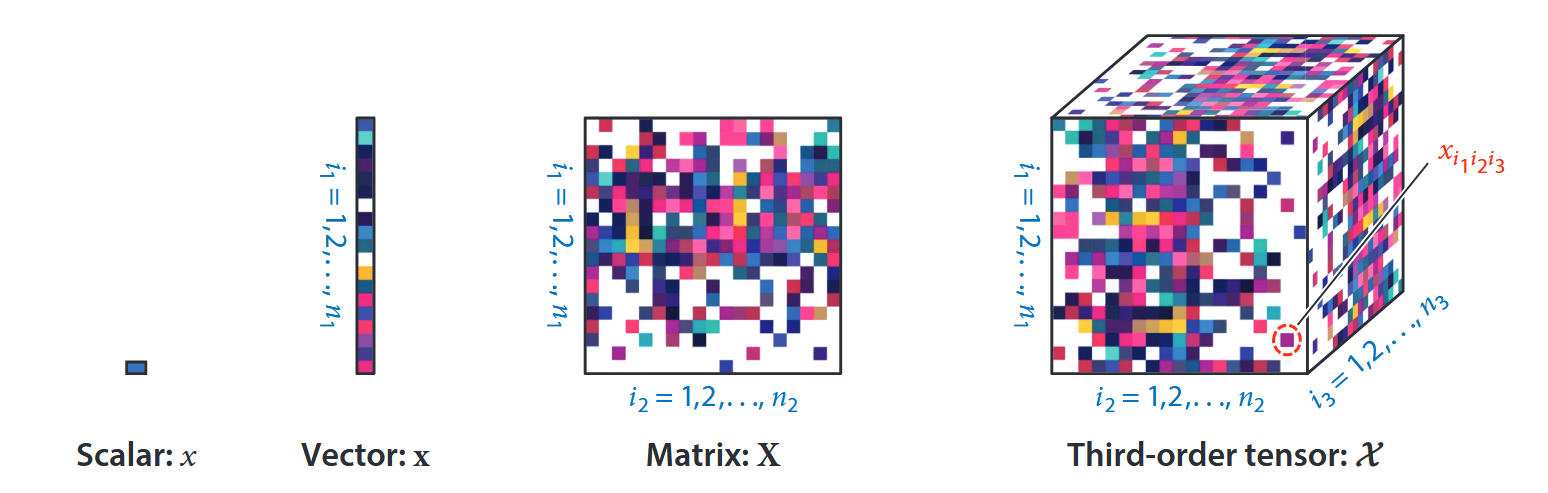
\includegraphics[width=0.8\columnwidth]{../figures/Example of Tensors.png}
	\caption{标量,向量,矩阵和三阶张量}
	\label{Fig:Example of Tensors}
\end{figure}

张量分解是一种将高维张量分解为若干低维因子组合的技巧,其中一种为Tucker分解\scite{tucker1966some},它是张量的高阶主成分分析(PCA),将张量分解为核心张量与各模式因子矩阵的乘积。具体地,给定一个张量$\mathcal{X} \in \mathbb{R}^{n_1 \times n_2 \times \cdots \times n_d}$,Tucker分解表示为:
\begin{equation}
	\mathcal{X} \approx \mathcal{C} \times_1 Q^1 \times_2 Q^2 \cdots \times_d Q^d = \sum_{j_1=1}^{m_1} \sum_{j_2=1}^{m_2} \cdots \sum_{j_d=1}^{m_d} c_{j_1 j_2 \dots j_d} 
	\, \mathbf{q}^{1}_{j_1} \circ \mathbf{q}^{2}_{j_2} \circ \cdots \circ \mathbf{q}^{d}_{j_d} \label{Equation:Tucker}
\end{equation}
其中,$\mathcal{C}\in \mathbb{R}^{m_1 \times m_2 \times \cdots \times m_d}$是核心张量,$Q^{k} \in \mathbb{R}^{n_k \times m_k}$是因子矩阵。图 \ref{Fig:Tucker}\scite{bi2021tensors} 给出了Tucker分解的图示。
\begin{figure}[h]
	\small
	\centering
	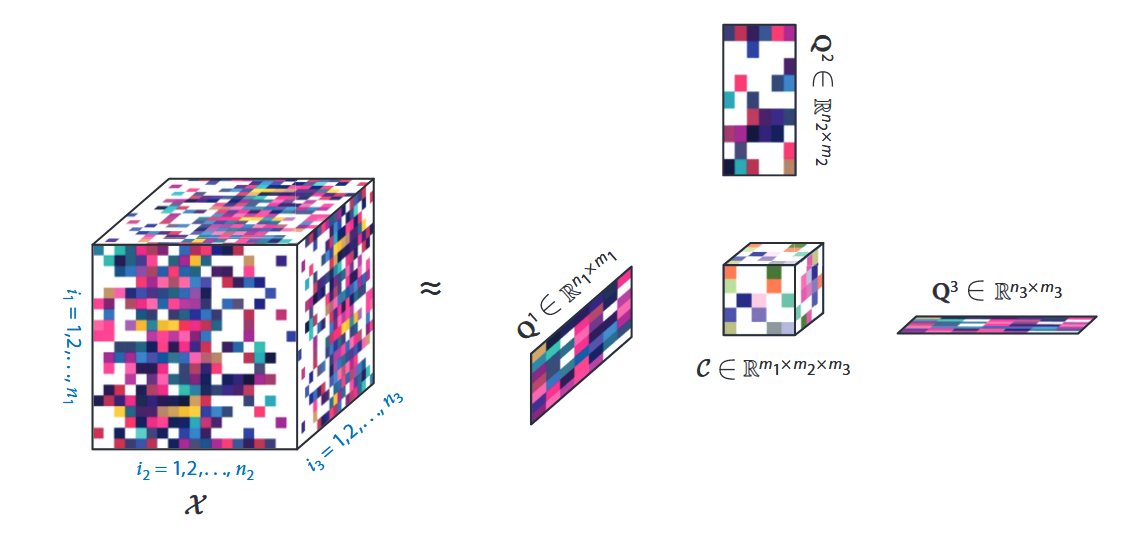
\includegraphics[width=0.8\columnwidth]{../figures/Tucker.png}
	\caption{Tucker分解}
	\label{Fig:Tucker}
\end{figure}
特别地,当$m_{1} =m_{2} = \cdots =m_{d} = R$,且核心张量限制为对角型时被称为PARAFAC分解。它将张量近似为一组秩为1的张量的和。具体而言,给定一个张量$\mathcal{X} \in \mathbb{R}^{n_1 \times n_2 \times \cdots \times n_d}$,其CP分解形式为:
\begin{equation}
	\mathcal{X} \approx \sum_{r=1}^{R} \boldsymbol{\beta}_1^{(r)} \circ \boldsymbol{\beta}_2^{(r)} \circ \cdots \circ \boldsymbol{\beta}_d^{(r)}
\end{equation}
其中$\boldsymbol{\beta}_{1},\cdots,\boldsymbol{\beta}_{d}$是长度为$p_{1},\cdots,p_{d}$的向量。PARAFAC分解将系数$p_{1}\times\cdots\times p_{d}$降低至$R(p_{1} + p_{2} +\cdots +p_{d})$,提供了有效的降维。

图 \ref{Fig:PARAFAC}\scite{bi2021tensors}提供了PARAFAC分解的简单图解。
\begin{figure}[h]
	\small
	\centering
	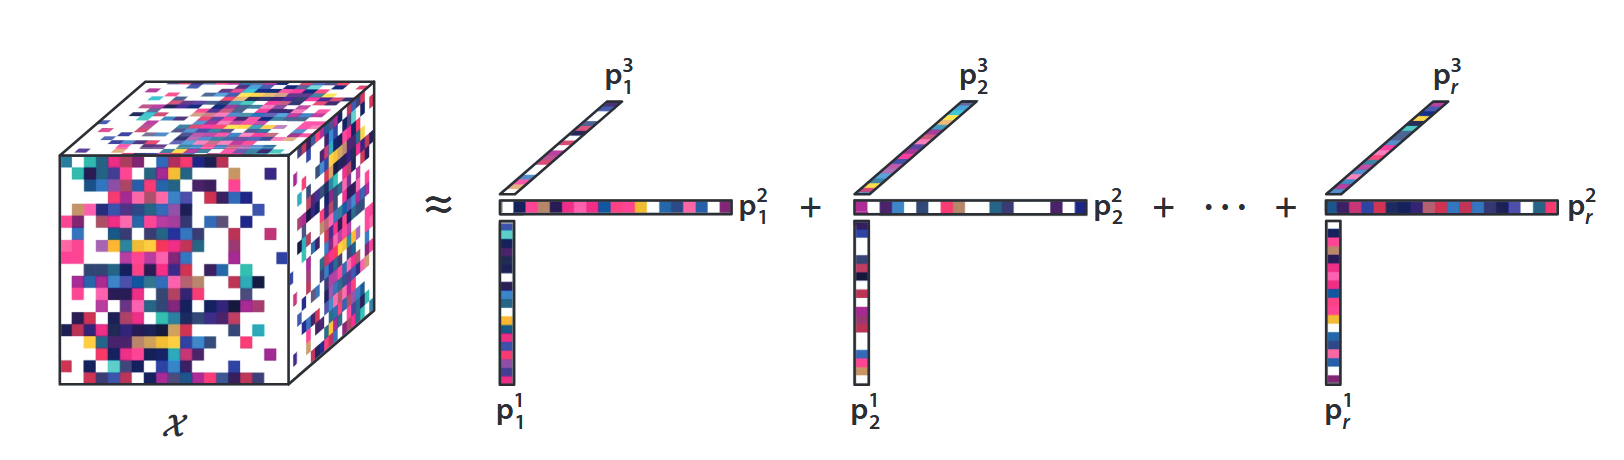
\includegraphics[width=\columnwidth]{../figures/PARAFAC.png}
	\caption{PARAFAC分解
	}
	\label{Fig:PARAFAC}
\end{figure}
\section{基于不同损失函数的分类模型}
损失函数就像是我们用来衡量“错误”的工具。在机器学习中,我们通过这个工具来评判模型训练性能。

贝叶斯方法中,损失函数转化为不同类型的似然(likelihood)。通过损失函数结合模型参数的先验假设和真实观测值来更新参数。通过这种方式,我们可以得到对模型参数的更好估计。

我们使用了两种常用的损失函数,分别是以支持向量机为代表的铰链损失(hinge loss)和逻辑回归损失(logistic regression loss),这两种损失函数都采用高维图像作为分类的协变量。

\subsection{支持向量机(SVM)}
大多数基于SVM的分类方法采用带惩罚项的点估计克服高维协变量的影响,通常有以下形式:
\begin{equation}
	\mathcal{L}(y|\boldsymbol{\beta}) = \dfrac{1}{\sigma^{2}}\text{max}(1-yf(\mathbf{x};\boldsymbol{\beta}),0) + R
	\label{Equation:Hinge Loss}
\end{equation}
这里的$y\in\{-1,1\}$是二元输出,$f(\cdot)$是协变量$\mathbf{x}$的线性或非线性函数,$\boldsymbol{\beta}$是需要从数据中估计的参数,以及$\sigma^{2}$是调整参数。图 \ref{Fig:Hinge Loss}给出了可视化的铰链损失。
\begin{figure}[h]
	\small
	\centering
	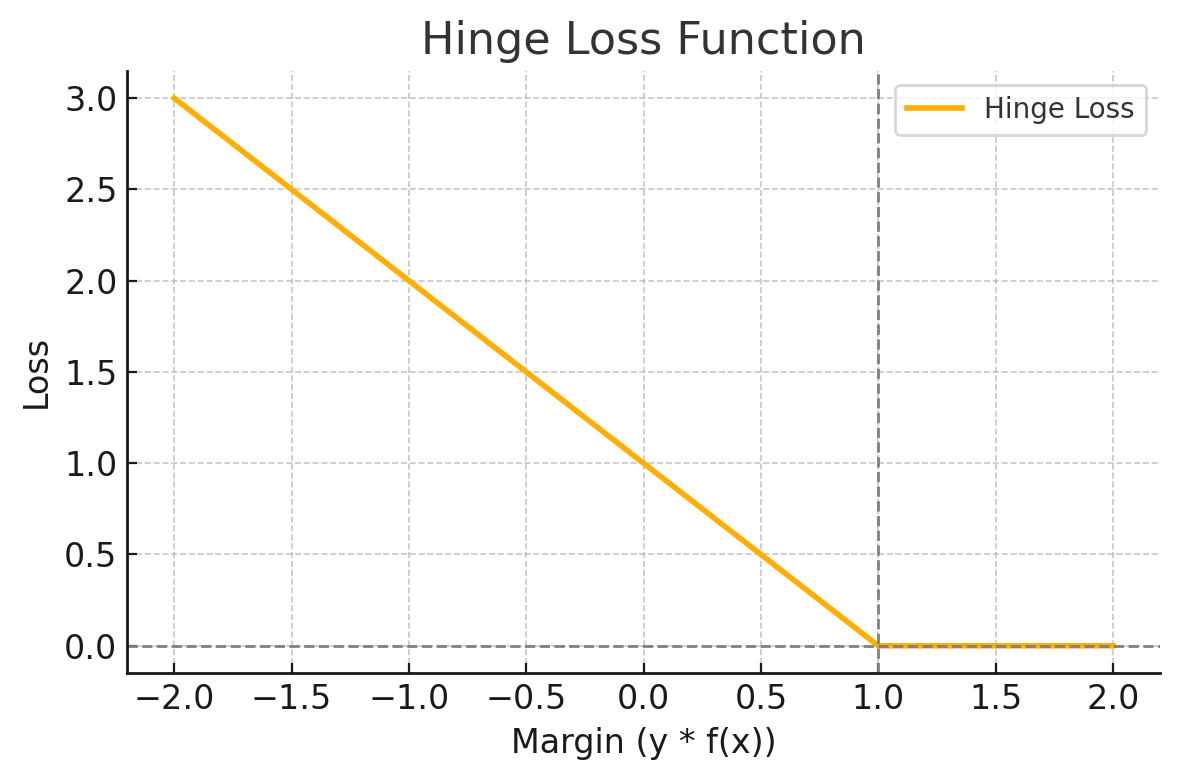
\includegraphics[width=0.6\columnwidth]{../figures/Hinge Loss.png}
	\caption{Hinge Loss
	}
	\label{Fig:Hinge Loss}
\end{figure}
SVM并没有明确的似然函数,不能直接在贝叶斯框架下建模。针对该问题,Polson 和 Scott提出了一种伪似然(pseudo-likelihood)的方法\scite{polson2011data}。

具体而言,伪似然可以被表示为一种带有潜在变量$\rho$的位置-尺度混合正态分布(location-scale mixture of normals):
\begin{align}
	L &= \prod_{i=1}^{n} L_{i}(y_{i}|\mathbf{x}_{i}, \boldsymbol{\beta}, \sigma^{2}) \notag 
	= \prod_{i=1}^{n} \left\{ \dfrac{1}{\sigma^{2}} \exp\{-\dfrac{2}{\sigma^{2}} \max\left(1 - y_{i} f(\mathbf{x}; \boldsymbol{\beta}), 0 \right)\} \right\}\notag \\
	&= \int_{0}^{\infty}\prod_{i=1}^{n}\dfrac{1}{\sigma\sqrt{2\pi\rho_{i}}}\exp(-\dfrac{(1+\rho_{i} - y_{i}f(\mathbf{x};\boldsymbol{\beta}))^{2}}{2\rho_{i}\sigma^{2}})\text{d}\rho_{i}
	\label{Equation:pseudo-likelihood}
\end{align}
这种表示法可以为后验推断提供高效的吉布斯采样器。
\subsection{逻辑回归(Logistic Regression)}
逻辑损失函数是一种S型损失,有如下形式:
\begin{equation}
	\mathcal{L}(y=1|\boldsymbol{\beta}) = \exp\{f(\mathbf{x};\boldsymbol{\beta})\}/(1+\exp\{f(\mathbf{x};\boldsymbol{\beta)}\})
\end{equation}
其中,$f(\mathbf{x};\boldsymbol{\beta})$代表协变量对逻辑损失的贡献。$\boldsymbol{\beta}$为待估参数. 图 \ref{Fig:Logistic Loss} 给出了可视化的损失函数。
\begin{figure}[h]
	\small
	\centering
	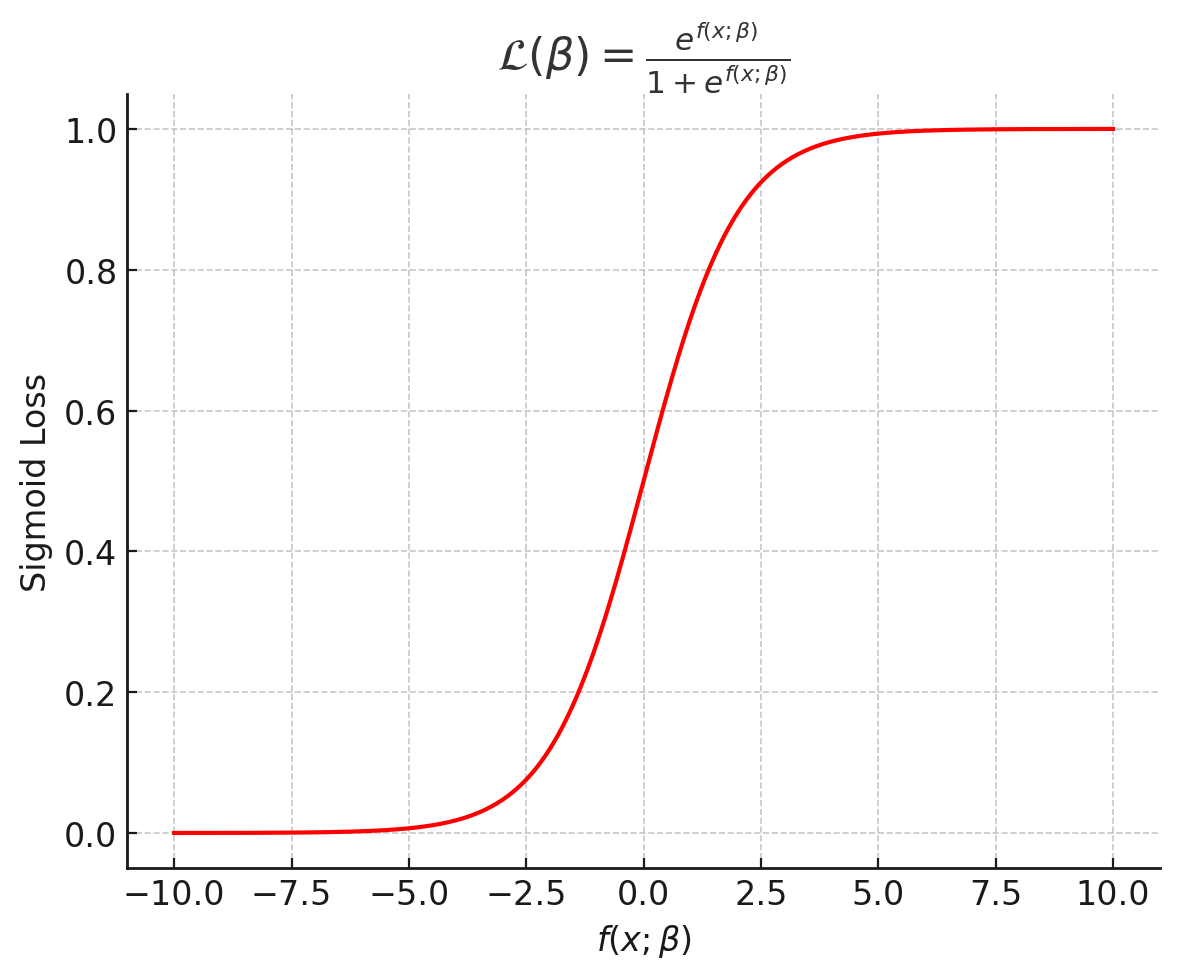
\includegraphics[width=0.6\columnwidth]{../figures/Logistic Loss.png}
	\caption{Logistic Loss
	}
	\label{Fig:Logistic Loss}
\end{figure}

在贝叶斯框架中,逻辑回归的似然函数在分析上并不方便处理,这使得直接从后验分布中采样变得困难。针对此问题,我们通常使用 Polya-Gamma 潜变量来实现\scite{polson2013bayesian}。 

	若随机变量$X$有如下形式
	\begin{equation}
		X \overset{D}{=} \dfrac{1}{2\pi^{2}}\sum_{k=1}^{\infty}\dfrac{g_{k}}{(k-1/2)^{2} + c^{2}/(4\pi^{2})
		}
		\label{PG}
	\end{equation}
	则称$X$服从参数为$b>0$, $c\in\mathbb{R}$的Polya-Gamma分布,记作$X\sim PG(b,c)$. 其中$g_{k}$服从Gamma分布$Ga(b,1)$,相互独立。$\overset{D}{=}$表示在分布意义下相等。


通过引入 Polya-Gamma 潜在变量可以将对数优势比参数化的二项式似然表示为关于 Polya-Gamma 分布的高斯混合\scite{polson2013bayesian}。

逻辑损失函数可以通过对潜在的 Polya-Gamma 变量进行边缘化处理而得到,其关系如下所示:
\begin{equation}
	\frac{(e^{f(\cdot)})^y}{(1 + e^{f(\cdot)})^b} = 2^{-b} e^{\kappa \psi} \int_0^\infty e^{-\omega \psi^2 / 2} p(\omega) \, d\omega,
	\quad b > 0, \quad \kappa = y - \frac{b}{2}
\end{equation}

其中 \( \omega \sim \text{PG}(b, 0) \),\( p(\omega) \) 表示 Polya-Gamma 分布的密度函数。

在该等式基础上,完整的数据增强似然函数为
\begin{equation}
	L = \prod_{i=1}^n \frac{(e^{f_i})^{y_i}}{1 + e^{f_i}} 
	= \prod_{i=1}^n 2^{-1} e^{\kappa_i \psi_i} \int_0^\infty e^{-\omega_i f_i^2 / 2} p(\omega_i) \, d\omega_i
\end{equation}

其中$\kappa_i = y_i - \frac{1}{2}$, $b = 1$, $\omega_i \sim \text{PG}(1, 0)$.

\section{先验估计}
我们采用广泛应用的线性预测模型
\begin{equation}
	f_{i} = \langle \mathbf{X}_{i}, \boldsymbol{B}\rangle + \mathbf{z}_{i}^{\prime}\boldsymbol{\gamma}
\end{equation}
这里的 \( \mathbf{X}_i \) 和 \( \mathbf{z}_i \) 分别表示第 \( i \) 个样本的影像预测变量与其他特征,例如人口统计学特征。  
符号 \( \langle \cdot, \cdot \rangle \) 表示内积算子。

张量系数矩阵 \( \boldsymbol{B} \) 用于量化图像在分类模型中的作用,  
\( \boldsymbol{\gamma} \) 是一个维度为 \( p_z + 1 \) 的向量,用以捕捉补充协变量的影响。

对张量$\boldsymbol{B}$进行PARAFAC分解,这里的
$\boldsymbol{B} \in \bigotimes_{j=1}^{d} \mathbb{R}^{p_j}$,有如下分解形式
\begin{equation}
	\boldsymbol{B} \approx \sum_{r=1}^{R} \boldsymbol{\beta}_1^{(r)} \circ \boldsymbol{\beta}_2^{(r)} \circ \cdots \circ \boldsymbol{\beta}_d^{(r)}
	\label{Equation:PARAFAC}
\end{equation}
在贝叶斯框架下需要有先验假设,对这里$\boldsymbol{\beta_{j}}^{(r)}$的先验选择,我们可以采用多向Dirichlet广义双帕累托(multiway Dirichlet generalized double Pareto ,M-DGDP)分布\scite{guhaniyogi2017bayesian}。

Guhaniyogi等人证明了\scite{guhaniyogi2017bayesian}使用该方法作为先验可以在贝叶斯张量回归中实现自动稀疏性控制、低秩建模与不失大信号的精确建模,同时具备对称性和后验一致性的理论保证。

具体地,该先验在各组分之间以可交换方式诱导收缩效应,其中全局尺度参数为 \( \tau \sim \mathrm{Ga}(a_\tau, b_\tau) \),并在每个组分中进行调整为 \( \tau_r = \phi_r \tau \),\( r = 1, \ldots, R \),其中
\begin{equation}
	\boldsymbol{\Phi} = (\phi_1, \ldots, \phi_R) \sim \mathrm{Dirichlet}(\alpha_1, \ldots, \alpha_R)
\end{equation}其作用是鼓励在假设的 PARAFAC 分解中向低秩方向收缩。

此外,令 \( \boldsymbol{W}_{jr} = \mathrm{diag}(w_{jr,1}, \ldots, w_{jr, p_j}) \),\( j = 1, \ldots, d \) 且 \( r = 1, \ldots, R \) 表示边缘特异的尺度参数。

层次结构的边缘层先验给定如下:
\begin{equation}
	\boldsymbol{\beta}^{(r)}_j \sim \mathcal{N}(0, (\phi_r \tau) \boldsymbol{W}_{jr}), 
	\quad w_{jr,k} \sim \mathrm{Exp}(\lambda_{jr}^2 / 2), 
	\quad \lambda_{jr} \sim \mathrm{Ga}(a_\lambda, b_\lambda).
	\label{Equation:prior}
\end{equation}

对元素特异尺度进行边缘化后,可得:
\begin{equation}
	\beta^{(r)}_{j,k} \mid \lambda_{jr}, \phi_r, \tau \overset{\text{iid}}{\sim} \mathrm{DE}(\lambda_{jr} / \sqrt{\phi_r \tau}), \quad 1 \leq k \leq p_j.
\end{equation}

式 \eqref{Equation:prior} 在单个边缘系数上诱导了 GDP(广义双帕累托)先验,从而具有自适应 Lasso 惩罚的形式。

在估计集合 \( \boldsymbol{B}_r = \{ \boldsymbol{\beta}_j^{(r)}; 1 \leq j \leq D \} \) 时,该模型通过引入边缘内异质性建模方式进行适应性调整,即引入元素特异的尺度参数 \( w_{jr,k} \). 其中共享的速率参数 \( \lambda_{jr} \) 可在边缘内的多个元素间传递信息,从而在局部尺度上诱导收缩。

最后我们假设$\gamma$的先验是$\mathcal{N}(0,\Sigma_{0\gamma})$,完成了所有参数的先验估计。

\section{后验推断的MCMC算法}
\subsection{MCMC算法简介\scite{李航2019统计学习方法}}
蒙特卡罗法(Monte Carlo method)是通过从概率模型的随机抽样进行近似数值计算的方法。 马尔可夫链蒙特卡罗法(Markov Chain Monte Carlo, MCMC),则是以马尔可夫链(Markov chain)为概率模型的蒙特卡罗法。

假设多元随机变量 $x$,满足 $x \in \mathcal{X}$,其概率密度函数为 $p(x)$,$f(x)$ 为定义在 $x \in \mathcal{X}$ 上的函数,目标是获得概率分布 $p(x)$ 的样本集合,以及求函数 $f(x)$ 的数学期望 $\mathbb{E}_{p(x)}[f(x)]$。

在随机变量 $x$ 的状态空间 $\mathcal{S}$ 上定义一个满足遍历定理的马尔可夫链 $X = \{X_0, X_1, \cdots, X_t, \cdots\}$,使其平稳分布就是抽样的目标分布 $p(x)$. 然后在这个马尔可夫链上进行随机游走,每个时刻得到一个样本。根据遍历定理,当时间足够长时(时刻大于某个正整数 $m$),在之后的时间(时刻小于等于某个正整数 $n,\ n > m$)里随机游走得到的样本集合 $\{x_{m+1}, x_{m+2}, \cdots, x_n\}$ 就是目标概率分布的抽样结果,得到的函数均值(遍历均值)就是要计算的数学期望值:

\begin{equation}
	\hat{f} = \frac{1}{n - m} \sum_{i = m+1}^{n} f(x_i) 
\end{equation}
到时刻 $m$ 为止的时间段称为燃烧期。

MCMC在贝叶斯学习中起重要的作用。
假设观测数据由随机变量 $y \in \mathcal{Y}$ 表示,模型由随机变量 $x \in \mathcal{X}$ 表示,贝叶斯学习通过贝叶斯定理计算给定数据条件下模型的后验概率,并选择后验概率最大的模型。

后验概率有如下计算公式:

\begin{equation}
	p(x|y) = \frac{p(x)p(y|x)}{\int_{\mathcal{X}} p(y|x')p(x') dx'} \label{Equation:posterior}
\end{equation}

贝叶斯学习中经常需要进行三种积分运算:归一化(normalization)、边缘化(marginalization)、数学期望(expectation)。

后验概率计算中需要归一化计算:

\begin{equation}
	\int_{\mathcal{X}} p(y|x')p(x') dx' \label{Equation:normalization}
\end{equation}

如果有隐变量 $z \in \mathcal{Z}$,后验概率的计算需要边缘化计算:

\begin{equation}
	p(x|y) = \int_{\mathcal{Z}} p(x, z|y) dz \label{Equation:marginalization}
\end{equation}

如果有一个函数 $f(x)$,可以计算该函数的关于后验概率分布的数学期望:

\begin{equation}
	\mathbb{E}_{P(x|y)}[f(x)] = \int_{\mathcal{X}} f(x) p(x|y) dx \label{Equation:expectation}
\end{equation}

当观测数据和模型都很复杂的时候,以上的积分计算变得困难。马尔可夫链蒙特卡罗法为这些计算提供了一个通用的有效解决方案。

\subsection{吉布斯采样(Gibbs Sampling)算法简介\scite{李航2019统计学习方法}}
常用的MCMC算法有Metropolis-Hastings算法、吉布斯采样法。

吉布斯抽样(Gibbs sampling)用于多元变量联合分布的抽样和估计。 其基本做法是,从联合概率分布定义满足条件概率分布,依次对满足条件概率分布进行抽样,得到样本的序列。可以证明这样的抽样过程是在一个马尔可夫链上的随机游走,每一个样本对应着马尔可夫链的状态,平稳分布就是目标的联合分布。整体成为一个马尔可夫链蒙特卡罗法,燃烧期之后的样本就是联合分布的随机样本。算法 \ref{Al:Gibbs} 中列出了具体的过程。
\begin{algorithm}[H]
	\caption{Gibbs Sampling(吉布斯抽样)}
	\label{Al:Gibbs}
	\begin{algorithmic}[1]
		\Require 目标分布的密度函数 $p(x)$,函数 $f(x)$;收敛步数 $m$,迭代步数 $n$
		\Ensure 随机样本 $\{x_{m+1}, \dots, x_n\}$ 及函数样本均值 $f_{mn}$
		
		\State 初始化:设初始样本 $x^{(0)} = (x_1^{(0)}, x_2^{(0)}, \dots, x_k^{(0)})^\top$
		\For{$i = 1$ to $n$}
		\State 设上一步样本为 $x^{(i-1)} = (x_1^{(i-1)}, x_2^{(i-1)}, \dots, x_k^{(i-1)})^\top$
		\For{$j = 1$ to $k$}
		\State 从条件分布 $p(x_j | x_1^{(i)}, \dots, x_{j-1}^{(i)}, x_{j+1}^{(i-1)}, \dots, x_k^{(i-1)})$ 中采样,得到 $x_j^{(i)}$
		\EndFor
		\State 得到当前样本 $x^{(i)} = (x_1^{(i)}, x_2^{(i)}, \dots, x_k^{(i)})^\top$
		\EndFor
		\State 抽取后 $n - m$ 个样本组成样本集合 $\{x^{(m+1)}, \dots, x^{(n)}\}$
		\State 计算函数样本均值:
		\[
		f_{mn} = \frac{1}{n - m} \sum_{i = m+1}^{n} f(x^{(i)})
		\]
	\end{algorithmic}
\end{algorithm}	

\subsection{基于SVM损失的贝叶斯张量模型}
令 \( y \in \mathbb{R} \) 表示一个响应值,  \( \mathbf{z} \in \mathbb{R}^p \), \( \mathbf{X} \in \bigotimes_{j=1}^{d} \mathbb{R}^{p_j} \)
,我们有如下的张量回归模型:
\begin{align}
	&y | \boldsymbol{\gamma}, \boldsymbol{B}, \sigma \sim \mathcal{N}(z^\prime \boldsymbol{\gamma} + \langle X, \boldsymbol{B} \rangle, \sigma^2) \notag \\
	&\boldsymbol{B} = \sum_{r=1}^{R} \boldsymbol{B}_r, \quad \boldsymbol{B}_r = \beta^{(r)}_1 \circ \cdots \circ \beta^{(r)}_d \notag \\
	&\boldsymbol{\gamma} \sim \pi_\gamma, \quad \beta^{(r)}_j \sim \pi_\beta \label{Equations:bayes-model}
\end{align}
先前提出的多向先验\eqref{Equation:prior} 可为张量回归模型 \eqref{Equations:bayes-model} 的大多数参数提供吉布斯采样方案。具体见算法 \ref{Al:BTSVM}。

\begin{algorithm}
	\caption{BT-SVM算法}
	\label{Al:BTSVM}
	\begin{algorithmic}[1]
		\State 从逆高斯分布更新 $\rho_i$: $\rho_i^{-1} \sim IN(\mu_i, \lambda_i)$, 其中 $\mu_i = |1 - y_i(<X_i, B> + z_i'\gamma)|^{-1}$ 且 $\lambda_i = 1/\sigma^2$.
		\State 对 $[\alpha, \boldsymbol{\Phi}, \tau | \boldsymbol{B}, \boldsymbol{W}]$ 组合采样为$[\alpha|\boldsymbol{B},\boldsymbol{W}][\boldsymbol{\Phi},\tau|\alpha, \boldsymbol{B},\boldsymbol{W}]$:
		\begin{itemize}
			\item[(a)] 使用 griddy-Gibbs 采样 \( [\alpha \mid \boldsymbol{B}, \boldsymbol{W}] \):对每个 \( \alpha \in \mathcal{A} \),通过从
			\( [\boldsymbol{\Phi}, \tau \mid \alpha, \boldsymbol{B}, \boldsymbol{W}] \) 采样 \( M \) 次,构建参考集.
			令 \( w_{j,l} = \pi(\boldsymbol{B} \mid \alpha, \boldsymbol{\Phi}_l, \tau_l, \boldsymbol{W}) \pi(\boldsymbol{\Phi}_l, \tau_l \mid \alpha) \),
			其中 \( 1 \leq l \leq M \),
			\( p(\alpha \mid \boldsymbol{B}, \boldsymbol{W}) = \pi(\alpha) \sum_{l=1}^M w_{j,l}/M \),以及
			
			\[
			\Pr(\alpha = \alpha_j \mid -) = \frac{p(\alpha_j \mid \boldsymbol{B}, \boldsymbol{W})}{\sum_{\alpha \in \mathcal{A}} p(\alpha \mid \boldsymbol{B}, \boldsymbol{W})}
			\]
			
			\item[(b)] 对特定组分采样尺度参数 $[\boldsymbol{\Phi}, \tau|\alpha^{*},\boldsymbol{B},\boldsymbol{W}] = [\boldsymbol{\Phi}|\boldsymbol{B},\boldsymbol{W}][\tau|\boldsymbol{\Phi,\boldsymbol{B},\boldsymbol{W}}]$
			;设 $p_0 = \sum_j^d p_j$, $a_\tau = R\alpha$, $b_\tau = \alpha(R/v)^{1/d}$.
			\begin{itemize}
				\item [(1)]对每个 $r=1,\dots,R$,采样:
				$\psi_r \sim \text{giG}(\alpha - p_0/2, 2b_\tau, 2C_r)$,其中 $C_r = \sum_{j=1}^d \boldsymbol{\boldsymbol{\beta}}_j^{(r)\top} \boldsymbol{W}_{jr}^{-1} \boldsymbol{\boldsymbol{\beta}}_j^{(r)}$,
				$\phi_r = \psi_r / \sum_{l=1}^R \psi_l$.
				\item [(2)]$\tau \sim \text{giG}(a_\tau - Rp_0/2, 2b_\tau, 2 \sum_{r=1}^R D_r)$,其中 $D_r = C_r/\phi_r$.
			\end{itemize}
		\end{itemize}
		
		\State 使用回溯拟合程序采样 $\{\boldsymbol{\beta}_j^{(r)}, \omega_{jr}, \lambda_{jr}\}$,以生成跨分量的边际条件分布的序列抽样。
		\begin{itemize}
			\item [(a)]抽取 $[w_{jr}, \lambda_{jr} \mid \boldsymbol{\beta}_j^{(r)}, \phi_r, \tau] = [w_{jr} \mid \lambda_{jr}, \boldsymbol{\beta}_j^{(r)}, \phi_r, \tau][\lambda_{jr} \mid \boldsymbol{\beta}_j^{(r)}, \phi_r, \tau]$.
			\begin{itemize}
				\item [(1)]抽取 $\lambda_{jr} \sim \text{Ga}\left(a_{\lambda} + p_j, b_{\lambda} + \left\|\boldsymbol{\beta}_j^{(r)}\right\|_1 / \sqrt{\phi_r \tau}\right)$;
				\item [(2)]对于 $1 \le k \le p_j$,独立抽取 $w_{jr,k} \sim \text{giG}\left(\frac{1}{2}, \frac{\lambda_{jr}^2}{2}, \boldsymbol{\beta}_{j,k}^2 / (\phi_r \tau)\right)$.
			\end{itemize}
			\item [(b)]从多元正态分布: $\boldsymbol{\beta}_j^{(r)} \sim N(\mu_{jr}, \Sigma_{jr})$抽取, 其中
			$\mu_{jr} = \frac{\Sigma_{jr} H_j^{(r)T} \tilde{\boldsymbol{y}}}{\sigma^2}$, $\Sigma_{jr} = \left(\frac{H_j^{(r)T} H_j^{(r)}}{\sigma^2} + \frac{W_{jr}^{-1}}{\phi_r \tau}\right)^{-1}$.
			以及
			$$
			h_{i,j,k}^{(r)} = \sum_{d_1=1,\dots,d_d=1}^{p_1,\dots,p_d} I(d_j=k) x_{d_1,\dots,d_d} \left(\prod_{l \ne j} \boldsymbol{\beta}_{l,i_l}^{(r)}\right),
			$$
			$$
			\boldsymbol{H}_{i,j}^{(r)} = (h_{1,j,1}^{(r)}/\sqrt{\rho_1}, \dots, h_{i,j,p_j}^{(r)}/\sqrt{\rho_i})',
			$$
			$$
			\tilde{y}_i = \frac{y_i}{\sqrt{\rho_i}} (\rho_i + 1 - y_i(z_i'\gamma + \sum_{l \ne r} < X_i, B_l >))
			$$
		\end{itemize}
		
		\State 从共轭正态条件分布 $\gamma \sim N(\mu_\gamma, \Sigma_\gamma)$ 更新 $\gamma$,其中
		$
		\mu_\gamma = \Sigma_\gamma Z^T(\tilde{y}y\rho)$, $ \Sigma_\gamma = (G^T G/\sigma^2 + \Sigma_{0\gamma})^{-1},
		$
		以及 $\boldsymbol{G}_{i,p_z} = Z_{i,p_z}/\sqrt{\rho_i}$ 和 $\tilde{y}_i = \rho_i + 1 - y_i < X_i, B >$.
		
	\end{algorithmic}
\end{algorithm}
\newpage
\subsection{基于Logistic损失的贝叶斯张量模型}
\begin{algorithm}
	\caption{BT-LR算法}
	\label{Al:BTLR}
	\begin{algorithmic}[1]
		\State 从 Pólya-gamma 分布更新 $\omega_i$: $\omega_i \sim \text{PG}(1, <X_i, \boldsymbol{B}> + z_i^T\gamma)$.
		\State 对 $[\alpha, \boldsymbol{\Phi}, \tau | \boldsymbol{B}, \boldsymbol{W}]$ 组合采样为$[\alpha|\boldsymbol{B},\boldsymbol{W}][\boldsymbol{\Phi},\tau|\alpha, \boldsymbol{B},\boldsymbol{W}]$:
		\begin{itemize}
			\item[(a)] 使用 griddy-Gibbs 采样 \( [\alpha \mid \boldsymbol{B}, \boldsymbol{W}] \):对每个 \( \alpha \in \mathcal{A} \),通过从
			\( [\boldsymbol{\Phi}, \tau \mid \alpha, \boldsymbol{B}, \boldsymbol{W}] \) 采样 \( M \) 次,构建参考集.
			令 \( w_{j,l} = \pi(\boldsymbol{B} \mid \alpha, \boldsymbol{\Phi}_l, \tau_l, \boldsymbol{W}) \pi(\boldsymbol{\Phi}_l, \tau_l \mid \alpha) \),
			其中 \( 1 \leq l \leq M \),
			\( p(\alpha \mid \boldsymbol{B}, \boldsymbol{W}) = \pi(\alpha) \sum_{l=1}^M w_{j,l}/M \),以及
			
			\[
			\Pr(\alpha = \alpha_j \mid -) = \frac{p(\alpha_j \mid \boldsymbol{B}, \boldsymbol{W})}{\sum_{\alpha \in \mathcal{A}} p(\alpha \mid \boldsymbol{B}, \boldsymbol{W})}
			\]
			
			\item[(b)] 对特定组分采样尺度参数 $[\boldsymbol{\Phi}, \tau|\alpha^{*},\boldsymbol{B},\boldsymbol{W}] = [\boldsymbol{\Phi}|\boldsymbol{B},\boldsymbol{W}][\tau|\boldsymbol{\Phi,\boldsymbol{B},\boldsymbol{W}}]$
			;设 $p_0 = \sum_j^d p_j$, $a_\tau = R\alpha$, $b_\tau = \alpha(R/v)^{1/d}$.
			\begin{itemize}
				\item [(1)]对每个 $r=1,\dots,R$,采样:
				$\psi_r \sim \text{giG}(\alpha - p_0/2, 2b_\tau, 2C_r)$,其中 $C_r = \sum_{j=1}^d \boldsymbol{\boldsymbol{\beta}}_j^{(r)\top} \boldsymbol{W}_{jr}^{-1} \boldsymbol{\boldsymbol{\beta}}_j^{(r)}$,
				$\phi_r = \psi_r / \sum_{l=1}^R \psi_l$.
				\item [(2)]$\tau \sim \text{giG}(a_\tau - Rp_0/2, 2b_\tau, 2 \sum_{r=1}^R D_r)$,其中 $D_r = C_r/\phi_r$.
			\end{itemize}
		\end{itemize}
		
		\State 使用回溯拟合程序采样 $\{\boldsymbol{\beta}_j^{(r)}, \omega_{jr}, \lambda_{jr}\}$,以生成跨分量的边际条件分布的序列抽样。
		\begin{itemize}
			\item [(a)]抽取 $[w_{jr}, \lambda_{jr} \mid \boldsymbol{\beta}_j^{(r)}, \phi_r, \tau] = [w_{jr} \mid \lambda_{jr}, \boldsymbol{\beta}_j^{(r)}, \phi_r, \tau][\lambda_{jr} \mid \boldsymbol{\beta}_j^{(r)}, \phi_r, \tau]$.
			\begin{itemize}
				\item [(1)]抽取 $\lambda_{jr} \sim \text{Ga}\left(a_{\lambda} + p_j, b_{\lambda} + \left\|\boldsymbol{\beta}_j^{(r)}\right\|_1 / \sqrt{\phi_r \tau}\right)$;
				\item [(2)]对于 $1 \le k \le p_j$,独立抽取 $w_{jr,k} \sim \text{giG}\left(\frac{1}{2}, \frac{\lambda_{jr}^2}{2}, \boldsymbol{\beta}_{j,k}^2 / (\phi_r \tau)\right)$.
			\end{itemize}
			\item [(b)]从多元正态分布中抽取 $\boldsymbol{\beta}_j^{(r)}$: $\boldsymbol{\beta}_j^{(r)} \sim N(\mu_{jr}, \Sigma_{jr})$, 其中 $\mu_{jr} = \Sigma_{jr}(\Omega(H_j^{(r)})^T\tilde{y})$ 且 $\Sigma_{jr} = ((H_j^{(r)})^T\Omega H_j^{(r)} + W_{jr}^{-1}/(\phi_r\tau))^{-1}$, 其中 $\tilde{y} = \kappa/\omega$, $\kappa = (y_1 - N_1/2, \dots, y_n - N_n/2)$, $N_1 = \dots = N_n = 1$, 且 $\Omega$ 是一个对角矩阵,其对角线元素为 $\omega_i$'s.
		\end{itemize}
		
		\State 从共轭正态条件分布 $\gamma \sim N(\mu_\gamma, \Sigma_\gamma)$ 更新 $\gamma$, 其中
		$
		\mu_\gamma = \Sigma_\gamma Z^T(\tilde{y}\omega)$, $\Sigma_\gamma = (G^T G + \Sigma_{0\gamma}^{-1})^{-1},
		$
		以及 $G_{i,p_z} = Z_{i,p_z} * \sqrt{\omega_i}$ 且 $\tilde{y}_i = \kappa_i/\omega_i - <X_i, B>$.
		
	\end{algorithmic}
\end{algorithm}

\subsection{参数设置}
通过选择先验分布中合适的超参数值,可以获得良好的整体性能。
基于Guhaniyogi等人的研究\scite{guhaniyogi2017bayesian},我们将全局尺度 $\tau$ 的超先验参数设为 $a_\tau = 1$ 和 $b_\tau = \alpha R^{(1/d)}$,其中 $R$ 是假设的 PARAFAC 分解中的秩,并设置 $\alpha_1 = \dots = \alpha_R = 1/R$。对于共同速率参数 $\lambda_{jr}$,我们设置 $a_\lambda = 3$ 和 $b_\lambda = \sqrt[d]{a_\lambda}$. 

在 SVM 损失下,缩放参数 $\sigma^2$ 是一个固定参数,可以手动调整以获得最大的模型性能。Lyu等人\scite{lyu2024bayesian}测试了从 $0.1$ 到 $10$ 的几个调整参数 $\sigma^2$ 值,并选择 $\sigma^2 = 6$。为了确定拟合模型的秩,使用秩 $2-5$ 拟合了所提出的模型,并选择了使偏差信息准则 (DIC) 分数最小的秩。

\chapter{模拟数据研究}
\section{数据生成}
我们通过几种模拟设置来阐述方法的性能,并使用其他已有的方法进行比较,这些方法基于各种类型的生成数据集,包括几种类型的函数信号以及由 SVM 和逻辑损失函数生成的数据. 我们考虑了四种不同类型的张量系数 $\boldsymbol{B}$ 来生成二元结果,设置如下:

\textbf{场景 1} 在此设置中,张量 $\boldsymbol{B}$ 由秩 $R_0 = 3$ 和维度 $p = c(48, 48)$ 的秩-$R$ PARAFAC 分解构建。每个 $\boldsymbol{\beta}$ 边缘 $\boldsymbol{\beta}_j^{(r)}$ 都是从独立的二项分布 $Binomial(2, 0.2)$ 生成的。在构建张量之后,我们将张量 $\boldsymbol{B}$ 单元格的最大值设置为 1。图 \ref{fig:scene1} 展示了该场景的张量图像。
\begin{lstlisting}[language=R]
p <- c(48, 48)
R <- 3

# 构造 rank-R PARAFAC 张量
generate_parafac_tensor <- function(p, R, prob = 0.2, size = 2) {
	A_list <- list()
	B_list <- list()
	
	for (r in 1:R) {
		a_r <- rbinom(p[1], size = size, prob = prob)
		b_r <- rbinom(p[2], size = size, prob = prob)
		A_list[[r]] <- a_r
		B_list[[r]] <- b_r
	}
	
	tensor <- matrix(0, nrow = p[1], ncol = p[2])
	for (r in 1:R) {
		tensor <- tensor + outer(A_list[[r]], B_list[[r]])
	}
	
	# 标准化为最大值为1
	tensor <- tensor / max(tensor)
	return(tensor)
}

# 生成张量
set.seed(123)
Beta_tens <- generate_parafac_tensor(p = c(48, 48), R = 3)
\end{lstlisting}

\textbf{场景 2} 张量图像由秩 $R_0 = 3$ 的秩-$R$ PARAFAC 分解模拟。这里,我们没有从已知分布生成张量边缘,而是手动设置了 $\boldsymbol{\beta}_j^{(r)}$ 的每个值。图 \ref{fig:scene2} 展示了该场景的张量图像。

\begin{lstlisting}[language=R]
# 手动设置边缘向量
a1 <- rep(0, 48)
a1[38:48] <- 1
b1 <- rep(0, 48)
b1[5:12] <- 1

a2 <- rep(0, 48)
a2[38:48] <- 1
b2 <- rep(0, 48)
b2[33:43] <- 1

a3 <- rep(0, 48)
a3[5:12] <- 1
b3 <- rep(0, 48)
b3[c(5:12, 33:43)] <- 1

# 构造 PARAFAC 张量
Beta_tens <- outer(a1, b1) + outer(a2, b2) + outer(a3, b3)

\end{lstlisting}
\textbf{场景 3} 与从 PARAFAC 分解生成 2D 张量图像不同,张量系数 $\boldsymbol{B}$ 对于矩形区域设置为 1,否则为 0.非零元素约占总面积的 30\%。图 \ref{fig:scene3} 展示了该场景的张量图像。

\begin{lstlisting}[language=R]
Beta_tens <- matrix(0, 48, 48)
for (i in 15:40) {
	for (j in 10:35) {
		Beta_tens[i, j] <- 1
	}
}

\end{lstlisting}
\textbf{场景 4} 张量系数 $\boldsymbol{B}$ 对于圆形区域设置为 1,否则为 0。非零元素约占总面积的 10\%。图 \ref{fig:scene4} 展示了该场景的张量图像。

\begin{lstlisting}[language=R]
Beta_tens <- matrix(0, 48, 48)
# 圆的中心和半径
center_x <- 18
center_y <- 18
radius <- sqrt(0.10 * 48 * 48 / pi)

# 填充圆形区域为 1
for (i in 1:48) {
	for (j in 1:48) {
		# 计算 (i, j) 到圆心的距离
		if ((i - center_x)^2 + (j - center_y)^2 <= radius^2) {
			Beta_tens[i, j] <- 1
		}
	}
}

\end{lstlisting}
\begin{figure}[h!]
	\centering
	\begin{minipage}{0.24\textwidth}
		\centering
		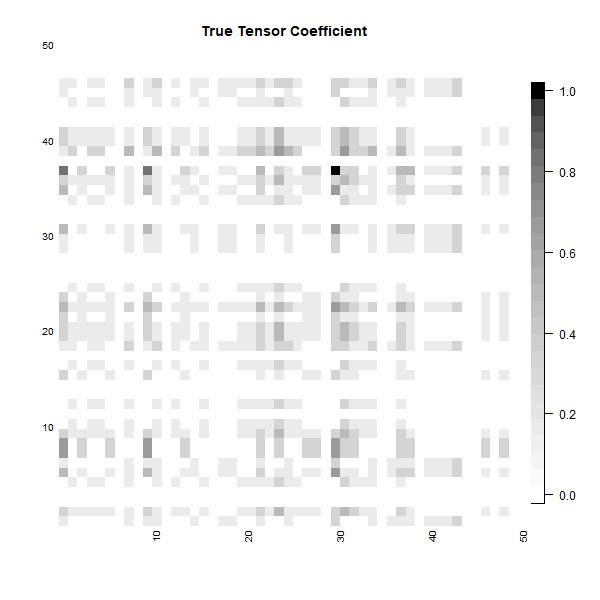
\includegraphics[width=\linewidth]{../figures/Beta_tens_Scenario1.png}
		\caption{Scene 1}
		\label{fig:scene1}
	\end{minipage}
	\hfill
	\begin{minipage}{0.24\textwidth}
		\centering
		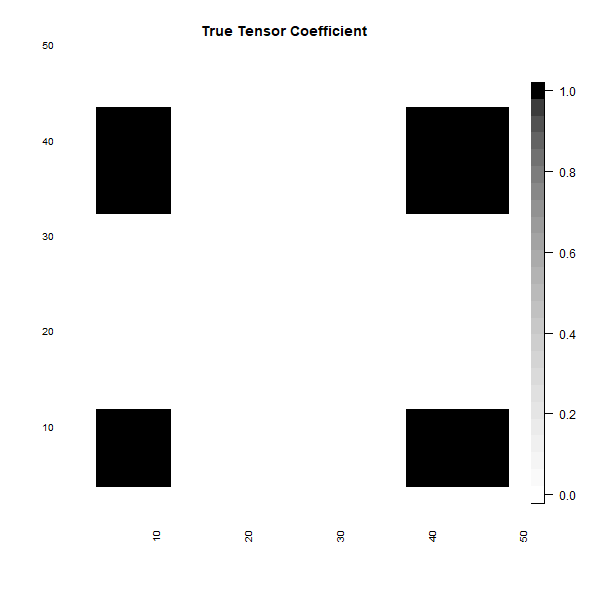
\includegraphics[width=\linewidth]{../figures/Beta_tens_Scenario2.png}
		\caption{Scene 2}
		\label{fig:scene2}
	\end{minipage}
	\hfill
	\begin{minipage}{0.24\textwidth}
		\centering
		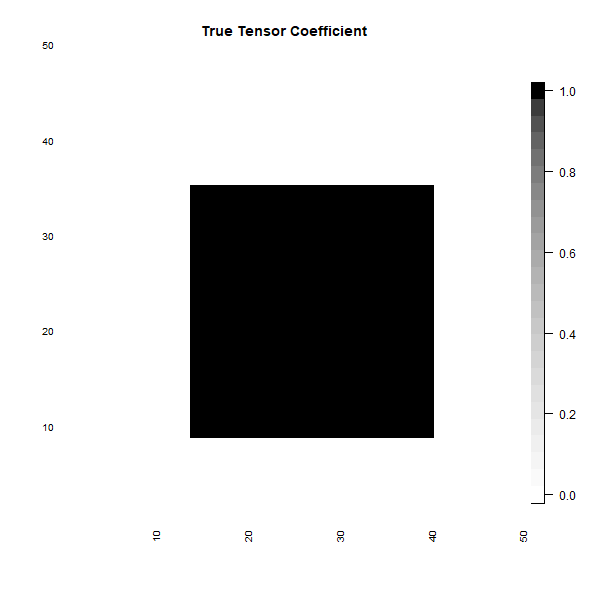
\includegraphics[width=\linewidth]{../figures/Beta_tens_Scenario3.png}
		\caption{Scene 3}
		\label{fig:scene3}
	\end{minipage}
	\hfill
	\begin{minipage}{0.24\textwidth}
		\centering
		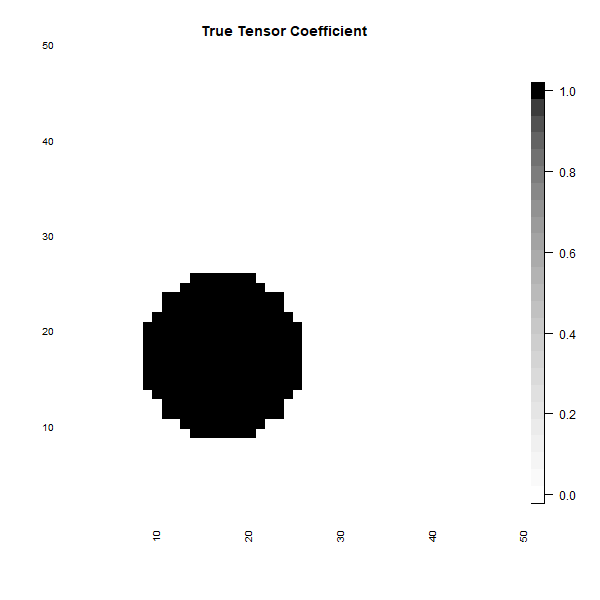
\includegraphics[width=\linewidth]{../figures/Beta_tens_Scenario4.png}
		\caption{Scene 4}
		\label{fig:scene4}
	\end{minipage}
\end{figure}

\section{模型评估}
我们使用均方根误差(Root Mean Squared Error, RMSE)与相关系数(correlation coefficient)来评估单元层级张量系数的点估计精度。同时,为了衡量分类准确性,我们计算误分类率(misclassification error)与 F1 分数(F1 score)。具体地,这些指标定义如下:

令 $\theta_j,~j=1,\dots,J$ 表示向量化的张量系数,其中 $J = \prod_{k=1}^d p_k$ 为张量系数 $\boldsymbol{B}$ 中的总单元数。此外,以下术语用于描述 SVM 分类器下的分类性能:
\begin{itemize}
	\item [(1)]真阳性(TP):分类器正确预测为阳性类别的样本数;
	\item [(2)]假阳性(FP):分类器将负类样本错误预测为阳性类别的样本数;
	\item [(3)]真阴性(TN):分类器正确预测为负类类别的样本数;
	\item [(4)]假阴性(FN):分类器将阳性样本错误预测为负类的样本数。
\end{itemize}

在逻辑回归模型中,以上定义相同,只是将负类替换为零类。此外,TP/FP/TN/FN 的定义亦可用于特征选择性能的评估,其中正类对应非零系数,而负类/零类则对应缺失或为零的系数。

\paragraph{系数估计性能指标} 包括以下两种:
\begin{itemize}
	\item[(1)] 均方根误差(Root-mean-square error),定义为:
	\begin{equation}
		\mathrm{RMSE}(\theta) = \sqrt{ \frac{1}{J} \sum_{j=1}^{J} (\hat{\theta}_j - \theta_j)^2 }
		\label{Equation:RMSE}
	\end{equation}
	用于衡量估计值与真实值之间的误差。
	\item[(2)] 估计系数与真实系数之间的相关系数。
\end{itemize}

\begin{lstlisting}[language=R]
tensor <- getBeta_mcmc(sim$beta.store)
tensor_est <- apply(tensor[burnin:nsweep, ], 2, mean) * sim$sy / sim$sx
rmse_val <- rmse(c(Beta_tens), c(tensor_est))
cor_val <- cor(c(Beta_tens), c(tensor_est))
\end{lstlisting}
\paragraph{分类性能指标} 包括:
\begin{itemize}
	\item[(i)] 误分类率(misclassification rate),定义为:
	\begin{equation}
		\frac{FP + FN}{TP + TN + FP + FN}
		\label{Equation:MisClaRate}
	\end{equation}
	
	\item[(ii)] F1 分数,定义为精确率(Precision)与召回率(Recall)的调和平均,其中:
	\begin{equation}
		\text{Precision} = \frac{TP}{TP + FP}, \quad \text{Recall} = \frac{TP}{TP + FN}
		\label{Equation:PrecisionandRecall}
	\end{equation}
	F1 分数表达式为:
	\begin{equation}
		\mathrm{F1} = \frac{2TP}{2TP + FP + FN}.
		\label{F1-score}
	\end{equation}
\end{itemize}

\begin{lstlisting}[language=R]
TP <- sum(clust.test == 1 & y.test == 1)
FP <- sum(clust.test == 1 & y.test == -1)
FN <- sum(clust.test == -1 & y.test == 1)N
f1score <- TP / (TP + (FP + FN) / 2)
\end{lstlisting}

实验中,我们将数据按 $70{:}30$ 的比例划分为训练集与测试集。用于系数估计与特征选择性能评估的指标在训练集上计算,而分类性能指标在测试集上进行评估。
\begin{lstlisting}[language=R]
train_index <- sort(sample(1:N, 0.7 * N, replace = FALSE))
x.train <- X[train_index, , ]
y.train <- Ylabel[train_index]
x.test <- X[-train_index, , ]
y.test <- Ylabel[-train_index]
\end{lstlisting}

为检验新模型的性能,我们选取两种现有的先进分类方法作为对比模型:

\paragraph{带有 Lasso 惩罚项的逻辑回归模型(Lasso Logistic Regression)}

该模型通过在传统逻辑回归的损失函数中引入 L1 正则项以实现特征选择,其优化目标如下:
\begin{equation}
	\hat{\boldsymbol{\beta}} = \arg\min_{\boldsymbol{\beta}} \left\{ 
	-\frac{1}{n} \sum_{i=1}^{n} \left[ y_i \log p_i + (1 - y_i) \log (1 - p_i) \right] 
	+ \lambda \|\boldsymbol{\beta}\|_1 
	\right\}
	\label{Equation:Lasso}
\end{equation}

其中 \( p_i = \frac{1}{1 + e^{-\mathbf{x}_i^\top \boldsymbol{\beta}}} \),
\(\lambda\) 为正则化参数,\(\|\boldsymbol{\beta}\|_1 = \sum_j |\beta_j|\) 表示 L1 范数。该模型由 R 语言中的 \texttt{glmnet} 包实现,适用于变量维度远高于样本数量的高维稀疏问题。
\begin{lstlisting}[language=R]
library(glmnet)
cvfit <- cv.glmnet(x.train.mat, y.train, family = "binomial", alpha = 1)
\end{lstlisting}

\paragraph{L1 范数支持向量机模型(L1-norm Support Vector Machine, SVM)}
该模型在传统支持向量机的基础上引入 L1 正则项,以增强特征选择能力,其优化目标函数如下:
\begin{equation}
	\hat{\boldsymbol{\beta}} = \arg\min_{\boldsymbol{\beta}} \left\{ 
	\frac{1}{2} \|\boldsymbol{\beta}\|_1 + C \sum_{i=1}^{n} \max(0, 1 - y_i \cdot \mathbf{x}_i^\top \boldsymbol{\beta}) 
	\right\}
	\label{Equation:L1SVM}
\end{equation}

其中 \( y_i \in \{-1, 1\} \),\(C\) 为调节间隔与误分类权衡的正则参数,第一项为 L1 范数惩罚项,第二项为 Hinge 损失函数。
该模型由 R 语言中的 \texttt{LiblineaR} 包实现,适用于高维低样本的稀疏分类任务。

\begin{lstlisting}[language=R]
library(LiblineaR)
model <- LiblineaR(data = x.train.mat, target = y.train, type = 5, cost = 1, bias = TRUE, verbose = FALSE)
\end{lstlisting}

这两种方法均基于张量协变量的向量化表示,将其转换为标量变量后输入统计模型中,因此无法保留张量图像的空间信息。
\begin{lstlisting}[language=R]
# 向量化
x.train.mat <- t(apply(x.train, 1, c))
x.test.mat <- t(apply(x.test, 1, c))
\end{lstlisting}
此外,我们还使用网格搜索算法与交叉验证来选择最佳调参值以进行模型拟合。

我们将MCMC链的迭代次数设置为3000,其中包含1000次的燃烧期,计算时间因所选的不同因素而有所不同。
\begin{table}[h!]
	\centering
	\caption{标签由SVM损失生成时不同模型在每种场景下的表现}
	\label{tab:performance_threeline SVM}
	\begin{tabular}{llcccc}
		\toprule 
		\textbf{Scenarios} & \textbf{Methods} & \textbf{RMSE} & \textbf{Corr.Coef.} & \textbf{Mis. Class.} & \textbf{F1-score} \\
		\midrule
		\multirow{4}{*}{Scenario 1} & LR w/ lasso & 0.186 & 0.118 & 0.500 & 0.576 \\
		& L1norm-SVM & 0.129 & 0.233 & 0.413 & 0.523 \\
		& BT-SVM & 0.127 & 0.591 & 0.340 & 0.653 \\
		& BT-LR & 0.197 & 0.449 & 0.360 & 0.640 \\
		
		\multirow{4}{*}{Scenario 2} & LR w/ Lasso & 0.395 & 0.057 & 0.520 & 0.487 \\
		& L1norm-SVM & 0.393 & 0.168 & 0.433 & 0.591 \\
		& BT-SVM & 0.285 & 0.820 & 0.193 & 0.803 \\
		& BT-LR & 0.330 & 0.505 & 0.347 & 0.653 \\
		
		\multirow{4}{*}{Scenario 3} & LR w/ Lasso & 0.541 & 0.064 & 0.453 & 0.585 \\
		& L1norm-SVM & 0.539 & 0.166 & 0.407 & 0.639 \\
		& BT-SVM & 0.430 & 0.768 & 0.227 & 0.788 \\
		& BT-LR & 0.454 & 0.570 & 0.320 & 0.684 \\
		
		\multirow{4}{*}{Scenario 4} & LR w/ Lasso & 0.315 & 0.178 & 0.407 & 0.639 \\
		& L1norm-SVM & 0.315 & 0.213 & 0.440 & 0.554 \\
		& BT-SVM & 0.221 & 0.769 & 0.207 & 0.805 \\
		& BT-LR & 0.276 & 0.529 & 0.347 & 0.679 \\
		\bottomrule
	\end{tabular}
\end{table}

表 \ref{tab:performance_threeline SVM} 和表 \ref{tab:performance_threeline Lasso} 中展示了评估模型性能的相关结果,分别对应场景1-4。具体而言,表 \ref{tab:performance_threeline SVM} 展示了在二元结果$Y$由SVM Loss生成时的四个场景的结果,而表 \ref{tab:performance_threeline Lasso} 则展示了当$Y$来自逻辑损失时的结果。这些结果表明,提出的两种方法(BT-SVM和BT-LR)在系数估计和分类性能上始终优于其他竞争的惩罚方法。

当二元结果数据来自SVM损失时:
\begin{lstlisting}[language=R]
# SVM Loss
Ylabel <- rep(0, N)
Ylabel[Y >= 0] <- 1
Ylabel[Y < 0] <- -1
\end{lstlisting}

BT-SVM方法具有优越的系数估计(如 表\ref{tab:performance_threeline SVM} 中较低的 RMSE 和较高的相关系数所示)和改进的分类精度(如表 \ref{tab:performance_threeline SVM} 中较低的误分类率和较高的F1分数所示)。即便在数据由逻辑损失生成时:
\begin{lstlisting}[language=R]
# Logistic loss
p <- 1 / (1 + exp(-Y))
Ylabel <- rbinom(n = N, size = 1, prob = p)
\end{lstlisting}依然有这一特点。
\begin{table}[h]
	\centering
	\caption{标签由逻辑损失生成时不同模型在每种场景下的表现}
	\label{tab:performance_threeline Lasso}
	\begin{tabular}{llcccc}
		\toprule
		\textbf{Scenarios} & \textbf{Methods} & \textbf{RMSE} & \textbf{Corr.Coef.} & \textbf{Mis. Class.} & \textbf{F1-score} \\
		\midrule
		\multirow{4}{*}{Scenario 1} & LR w/ lasso & 0.175 & 0.078 & 0.493 & 0.580 \\
		& L1norm-SVM & 0.192 & 0.208 & 0.527 & 0.448 \\
		& BT-SVM & 0.120 & 0.701 & 0.220 & 0.793 \\
		& BT-LR & 0.230 &  0.456 & 0.340 & 0.698 \\
		\midrule
		\multirow{4}{*}{Scenario 2} & LR w/ Lasso & 0.395 & 0.128 & 0.547 & 0.474 \\
		& L1norm-SVM & 0.393 & 0.215 & 0.453 & 0.534 \\
		& BT-SVM & 0.233 & 0.880 & 0.140 & 0.844 \\
		& BT-LR & 0.284 & 0.670 & 0.233 & 0.788 \\
		\midrule
		\multirow{4}{*}{Scenario 3} & LR w/ Lasso & 0.542 & 0.050 & 0.427 & 0.467 \\
		& L1norm-SVM & 0.539 & 0.149 & 0.413 & 0.544 \\
		& BT-SVM & 0.426 & 0.811 & 0.187 & 0.823 \\
		& BT-LR & 0.414 & 0.555 & 0.313 & 0.647 \\
		\midrule
		\multirow{4}{*}{Scenario 4} & LR w/ Lasso & 0.316 & 0.127 & 0.447 & 0.518 \\
		& L1norm-SVM & 0.315 & 0.193 & 0.473 & 0.530 \\
		& BT-SVM & 0.221 & 0.739 & 0.213 & 0.790 \\
		& BT-LR & 0.317 & 0.479 & 0.360 & 0.635 \\
		\bottomrule
	\end{tabular}
\end{table}

图 \ref{fig:all_scenarios} 展示了使用 BT-SVM 和 BT-LR 估算张量系数的情况。从图中可以看出,我们提出的方法能够广泛地恢复二维张量$\boldsymbol{B}$的形状,而不受其形状的影响,也不取决于张量信号是否通过PARAFAC分解构建。

\begin{figure}[h]
	\centering
	\begin{minipage}{0.24\textwidth}
		\centering
		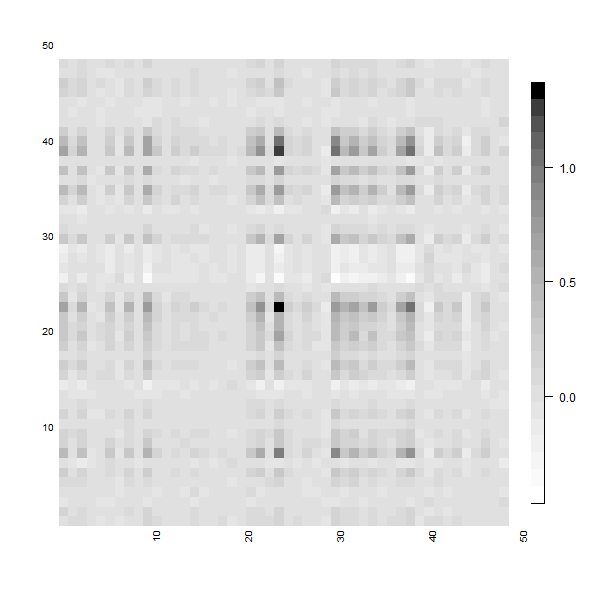
\includegraphics[width=\textwidth]{../figures/Tensor_estimated_Scenario1_SVM.png}
		\label{fig:scenario1_SVM}
	\end{minipage}
	\hfill
	\begin{minipage}{0.24\textwidth}
		\centering
		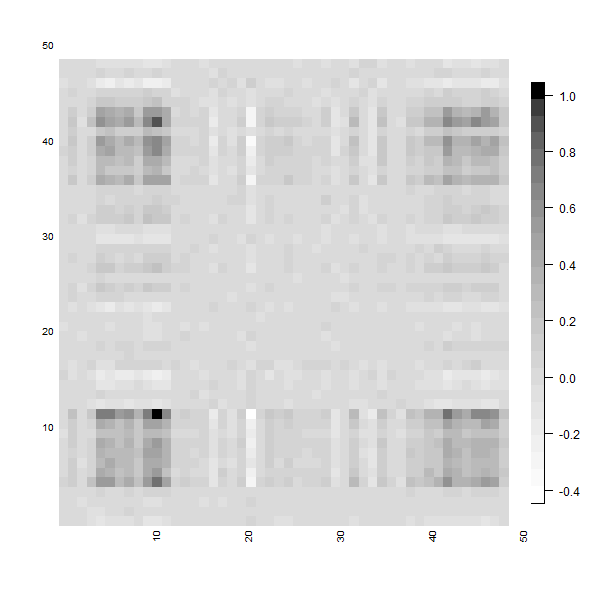
\includegraphics[width=\textwidth]{../figures/Tensor_estimated_Scenario2_SVM.png}
		\label{fig:scenario2_SVM}
	\end{minipage}
	\hfill
	\begin{minipage}{0.24\textwidth}
		\centering
		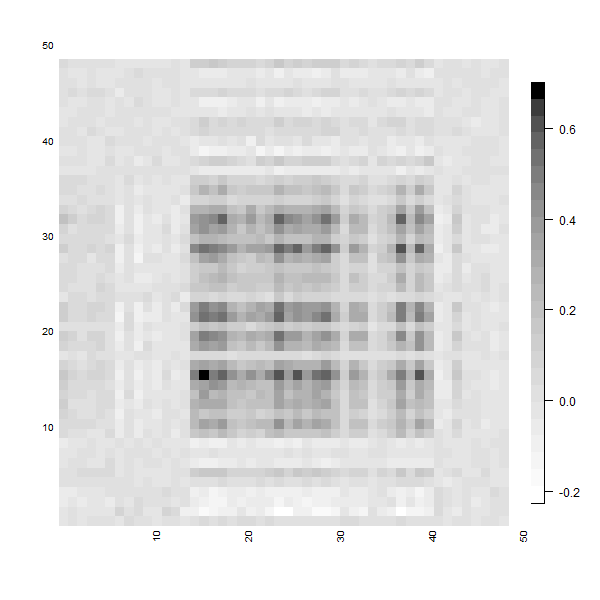
\includegraphics[width=\textwidth]{../figures/Tensor_estimated_Scenario3_SVM.png}
		\label{fig:scenario3_SVM}
	\end{minipage}
	\hfill
	\begin{minipage}{0.24\textwidth}
		\centering
		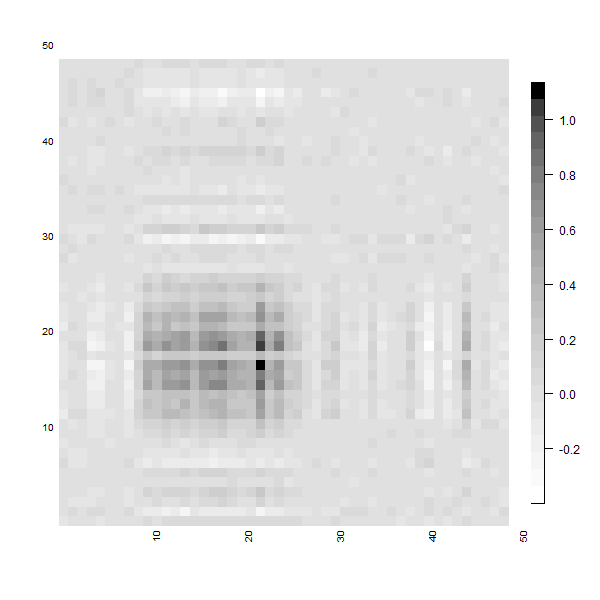
\includegraphics[width=\textwidth]{../figures/Tensor_estimated_Scenario4_SVM.png}
		\label{fig:scenario4_SVM}
	\end{minipage}
	
	
	\begin{minipage}{0.24\textwidth}
		\centering
		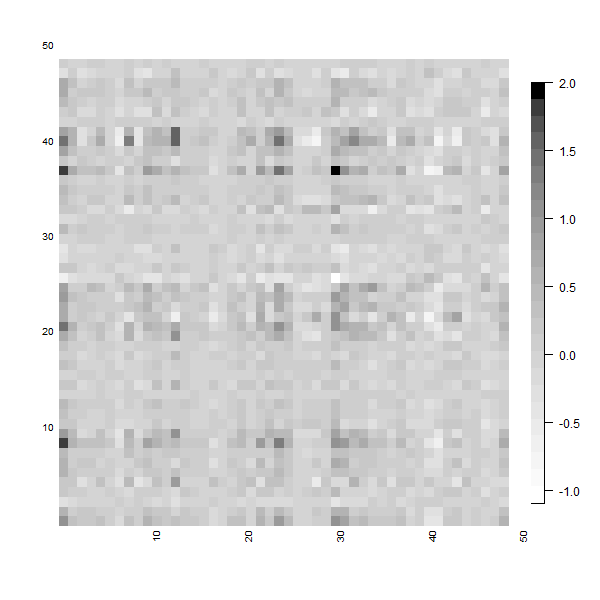
\includegraphics[width=\textwidth]{../figures/Tensor_estimated_Scenario1_LR.png}
		\label{fig:scenario1_LR}
	\end{minipage}
	\hfill
	\begin{minipage}{0.24\textwidth}
		\centering
		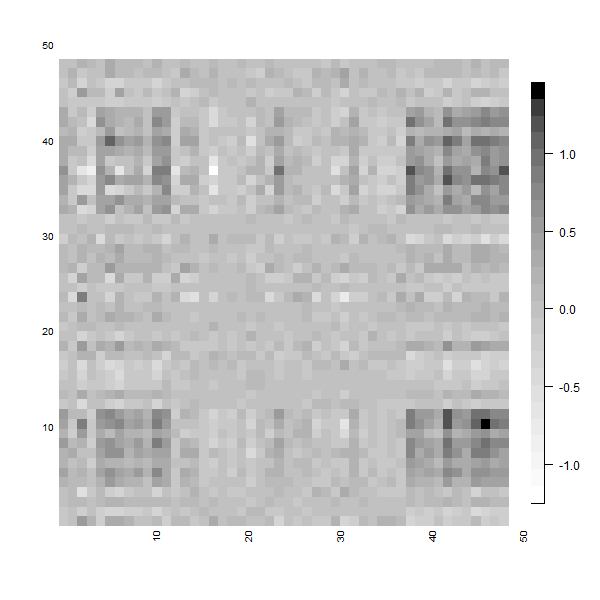
\includegraphics[width=\textwidth]{../figures/Tensor_estimated_Scenario2_LR.png}
		\label{fig:scenario2_LR}
	\end{minipage}
	\hfill
	\begin{minipage}{0.24\textwidth}
		\centering
		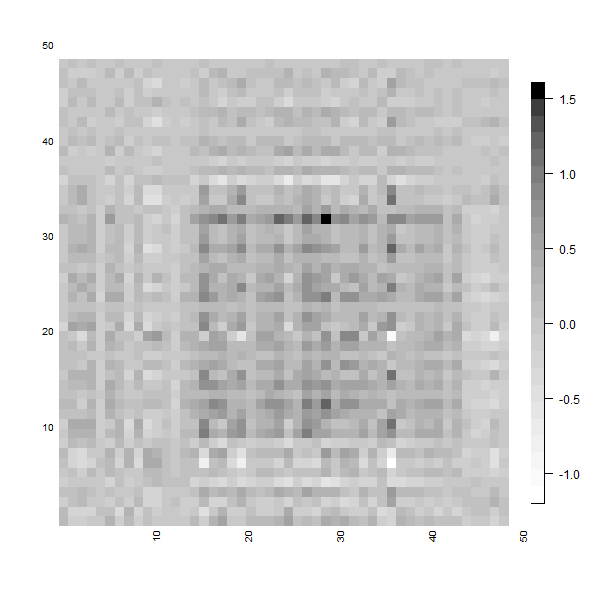
\includegraphics[width=\textwidth]{../figures/Tensor_estimated_Scenario3_LR.png}
		\label{fig:scenario3_LR}
	\end{minipage}
	\hfill
	\begin{minipage}{0.24\textwidth}
		\centering
		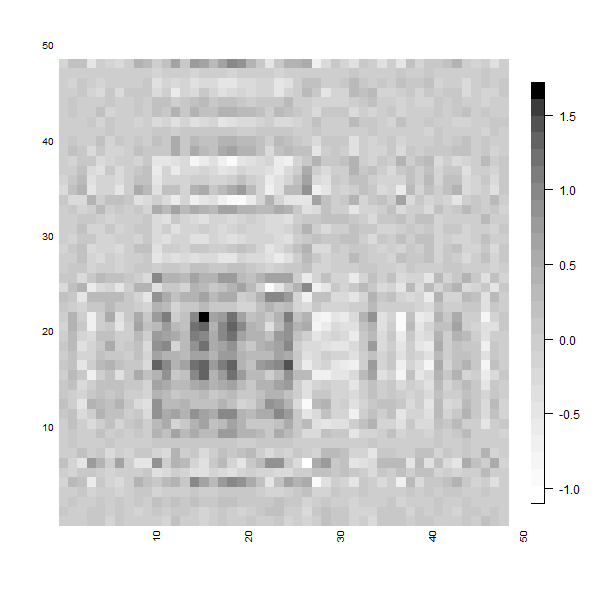
\includegraphics[width=\textwidth]{../figures/Tensor_estimated_Scenario4_LR.png}
		\label{fig:scenario4_LR}
	\end{minipage}
	
	\caption{估计的张量系数(第一排由BT-SVM模型估计 第二排由BT-LR模型估计)}
	\label{fig:all_scenarios}
\end{figure}
\begin{figure}[h]
	\centering
	\begin{minipage}{0.24\textwidth}
		\centering
		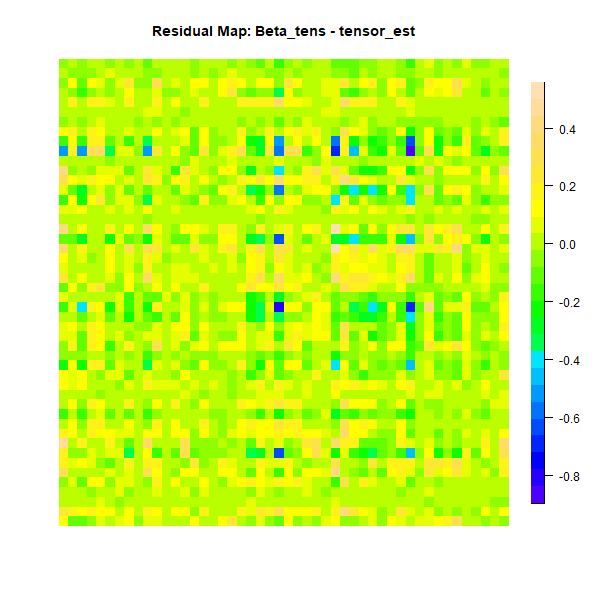
\includegraphics[width=\textwidth]{../figures/Residual_Tensor_Scenario1_SVM.png}
		\label{fig:residual_scenario1_SVM}
	\end{minipage}
	\hfill
	\begin{minipage}{0.24\textwidth}
		\centering
		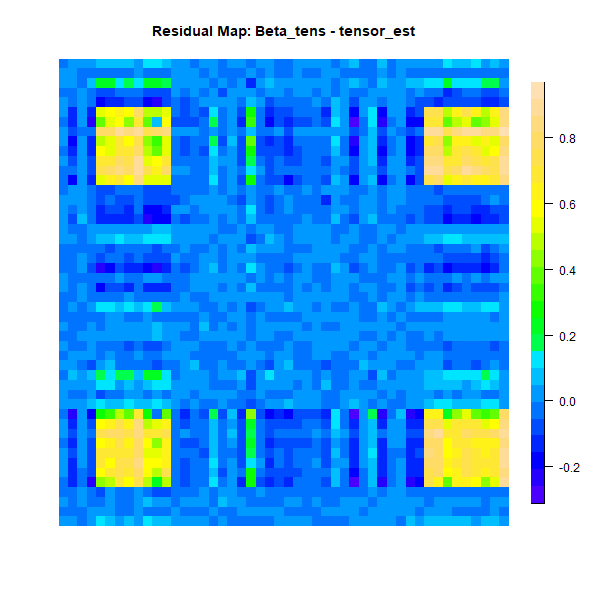
\includegraphics[width=\textwidth]{../figures/Residual_Tensor_Scenario2_SVM.png}
		\label{fig:residual_scenario2_SVM}
	\end{minipage}
	\hfill
	\begin{minipage}{0.24\textwidth}
		\centering
		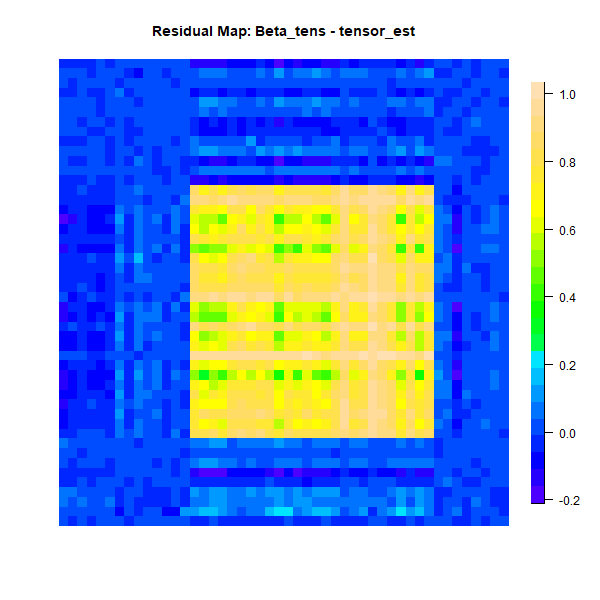
\includegraphics[width=\textwidth]{../figures/Residual_Tensor_Scenario3_SVM.png}
		\label{fig:residual_scenario3_SVM}
	\end{minipage}
	\hfill
	\begin{minipage}{0.24\textwidth}
		\centering
		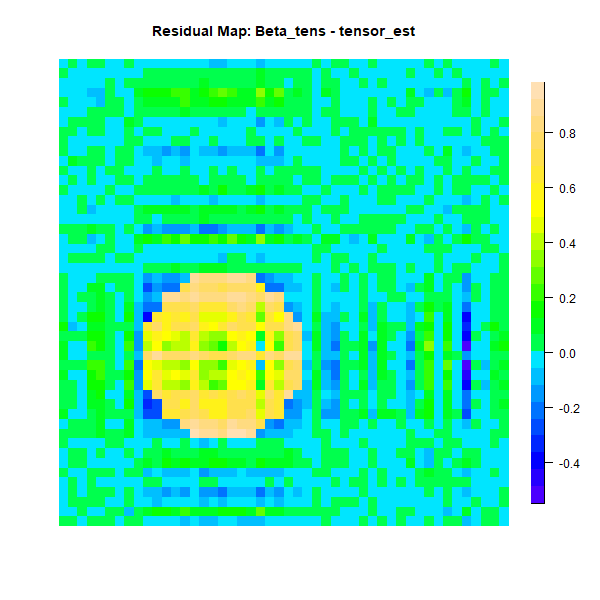
\includegraphics[width=\textwidth]{../figures/Residual_Tensor_Scenario4_SVM.png}
		\label{fig:residual_scenario4_SVM}
	\end{minipage}
	
	\begin{minipage}{0.24\textwidth}
		\centering
		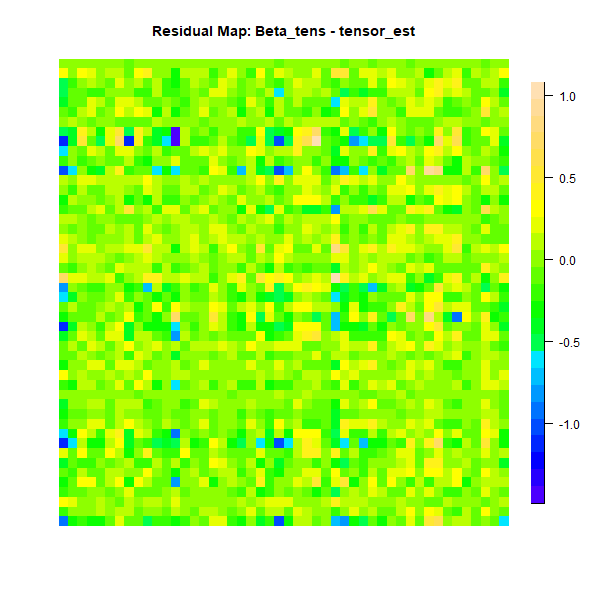
\includegraphics[width=\textwidth]{../figures/Residual_Tensor_Scenario1_LR.png}
		\label{fig:residual_scenario1_LR}
	\end{minipage}
	\hfill
	\begin{minipage}{0.24\textwidth}
		\centering
		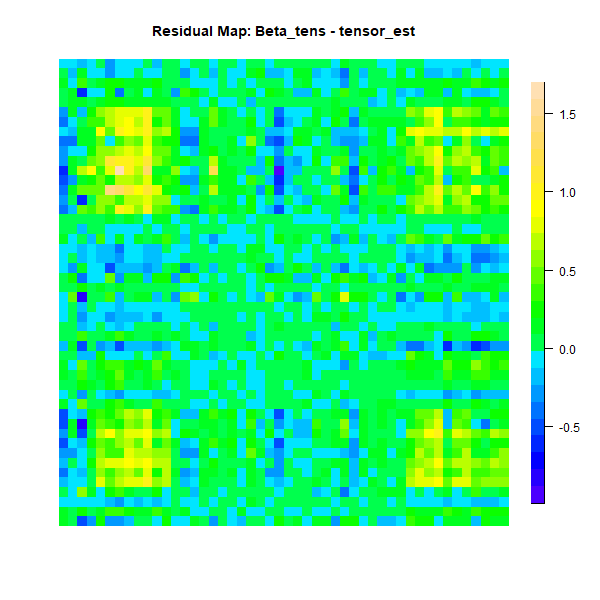
\includegraphics[width=\textwidth]{../figures/Residual_Tensor_Scenario2_LR.png}
		\label{fig:residual_scenario2_LR}
	\end{minipage}
	\hfill
	\begin{minipage}{0.24\textwidth}
		\centering
		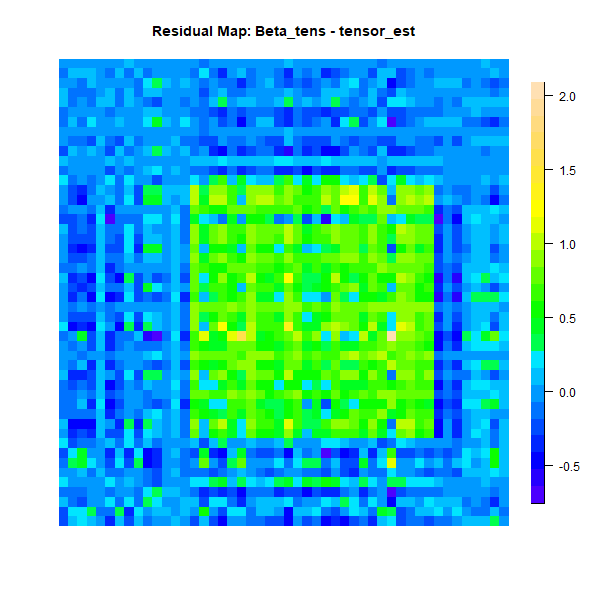
\includegraphics[width=\textwidth]{../figures/Residual_Tensor_Scenario3_LR.png}
		\label{fig:residual_scenario3_LR}
	\end{minipage}
	\hfill
	\begin{minipage}{0.24\textwidth}
		\centering
		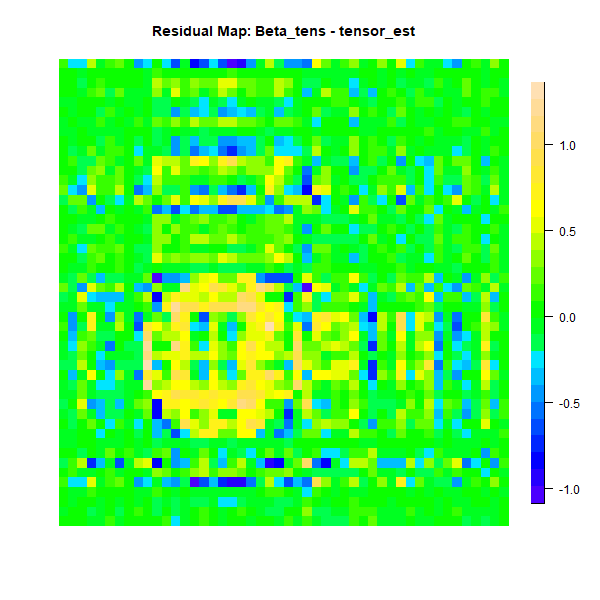
\includegraphics[width=\textwidth]{../figures/Residual_Tensor_Scenario4_LR.png}
		\label{fig:residual_scenario4_LR}
	\end{minipage}
	
	\caption{残差图}
	\label{fig:residual_maps_all}
\end{figure}
为了展示预测系数和真实系数之间的相关程度,我们通过图 \ref{fig:residual_maps_all} 展示了不同模型(LR 和 SVM)在不同情景下的表现. 

\begin{lstlisting}[language=R]
residual_map <- Beta_tens - matrix(tensor_est, nrow = 48)
png("Residual_Tensor_Scenario4_SVM.png", width = 600, height = 600)
image.plot(residual_map,
col = topo.colors(25), axes = FALSE,
main = "Residual Map: Beta_tens - tensor_est"
)
dev.off()
\end{lstlisting}
这些热力图展示了每个情景下模型预测值与真实值之间的残差分布,便于分析每个模型的准确性和误差特征。


相比之下,带惩罚项的竞争方法,例如带 LASSO 惩罚的逻辑回归和 L1norm-SVM)表现不佳。从表 \ref{tab:performance_threeline SVM} 和表 \ref{tab:performance_threeline Lasso} 中可以发现,真实系数和估计系数之间的相关系数往往接近于零,反映了它们无法检测到真实信号,从而导致系数估计性能不佳,分类效果大打折扣。

\section{MRI脑肿瘤分类}
为了进一步验证所提出模型的实际应用效能,本研究在一个包含脑部肿瘤切片MRI图像和正常MRI图像的数据集上进行了分类任务。该数据集共包含155张肿瘤图像和98张正常图像,为评估模型在真实医学影像场景下的性能提供了基础。为了确保评估的严谨性与普适性,我们将整个数据集按照70\%训练集与30\%测试集的比例进行随机划分。

考虑到该数据集的样本量相对较小,在进行MCMC算法进行后验推断时,我们将迭代次数设定为500次,其中燃烧期为200次。此外,为了适应张量模型的输入要求,原始图像数据被统一转换并构建为48x48像素的灰度张量信号,为高维数据的有效处理奠定了基础。

我们对比了四种分类模型在该任务上的表现,测试结果如表 \ref{tab:performance_threeline MRI}所示:

\begin{table}[h]
\centering
\caption{不同模型对脑肿瘤影像的分类性能}
\label{tab:performance_threeline MRI}
\begin{tabular}{llcccc}
\toprule
\textbf{Methods} & \textbf{Mis. Class.} & \textbf{F1-score} \\
\midrule
LR w/ lasso & 0.333 & 0.702  \\
L1norm-SVM & 0.451 & 0.709 \\
BT-SVM & 0.211 & 0.855 \\
BT-LR & 0.303 &  0.763  \\
\bottomrule
\end{tabular}
\end{table}

从表1的实验结果中可以观察到,在脑肿瘤MRI图像分类任务中,BT-SVM模型表现良好。其误分类率仅为0.211,显著低于所有其他对比模型;同时,其F1-分数高达0.855。相比之下,传统的带Lasso惩罚的逻辑回归模型和L1范数支持向量机模型的分类效果不及BT-SVM,尤其L1norm-SVM的误分类率甚至达到了0.451。

这一结果进一步表明传统的向量化处理而不考虑其空间结构信息的分类方法,在医学影像分析这类复杂任务中往往难以有效捕捉真实信号。而本研究所提出的贝叶斯张量模型通过张量分解有效保留并利用了图像的空间结构信息。这充分证明了贝叶斯张量分类模型在处理高维、具有复杂空间结构的医学影像数据方面的强大潜力,为未来脑部疾病的辅助诊断提供了有力的工具。
\backmatter

\printbib

\Appendix

\begin{lstlisting}[language=R, caption = {BT-SVM}算法]
library(fields)
library(abind)
library(imager)
library(magrittr)
SVMDPL <- function(Z, X, Ylabel, rank = 3, nsweep = 1e3, nskip = 3, a.lam, b.lam, phi.alpha, scale = TRUE) {
	library(base)
	library(statmod)
	library(MASS)
	library(matlib)
	library(stats)
	library(plyr)
	library(GIGrvg)
	library(gtools)
	library(coda)
	library(fields)
	library(dplyr)
	
	## data input
	# N : 样本数量
	# P: 张量图像大小,例如 48*48
	# D: 张量图像的维度数,对于二维张量,D=2; 对于三维张量,D=3.
	# Z : 一个包含人口统计协变量的 N 行 pgamma 列 矩阵(例如,年龄、性别等信息) pgamma是协变量的数量。
	# X  : N *  P[1] * P[2] 图像数据张量,N 个 P[1] * P[2] 大小的图像。
	# Ylabel : 包含二分类标签的相应变量。
	
	# 初始化变量 
	Yi <- Ylabel
	N <- length(Yi)
	P <- dim(X)[-1]
	D <- length(dim(X)) - 1
	pgamma <- ncol(Z)
	
	# 标准化
	if (is.null(Z)) {
		mz <- NA
		sz <- NA
	} else {
		mz <- colMeans(Z)
		sz <- rep(1, pgamma)
	}
	if (!is.null(Z)) {
		if (!is.matrix(Z)) {
			Z <- as.matrix(Z)
		}
	}
	Zt <- Z
	obs <- as.numeric(Yi)
	sy <- 1
	my <- 0
	
	if (scale) {
		if (!is.null(Z)) {
			mz <- colMeans(Z)
			sz <- apply(Z, 2, function(z) diff(range(z)))
			sz[sz == 0] <- 1
			Zt <- Z
			for (jj in 1:pgamma) {
				Zt[, jj] <- (Z[, jj] - mz[jj]) / sz[jj]
			}
		}
		Xt <- 0 * X
		mx <- apply(X, c(2:(D + 1)), function(z) mean(z, na.rm = T))
		sx <- apply(X, c(2:(D + 1)), function(z) diff(range(z, na.rm = T)))
		sx[sx == 0] <- 1
		if (D == 2) {
			for (jj in 1:nrow(X)) Xt[jj, , ] <- (X[jj, , ] - mx) / sx
		} else if (D == 3) {
			for (jj in 1:nrow(X)) Xt[jj, , , ] <- (X[jj, , , ] - mx) / sx
		}
	} else {
		if (!is.null(Z)) {
			mz <- rep(0, pgamma)
			sz <- rep(1, pgamma)
			Zt <- Z
		}
		mx <- array(0, dim = dim(X)[-1])
		sx <- array(1, dim = dim(X)[-1])
		Xt <- X
	}
	
	# MCMC setup

	x.train.nona <- Xt
	x.train.nona[is.na(Xt)] <- 0
	
	if (missing(a.lam)) a.lam <- rep(3, rank)
	if (missing(b.lam)) b.lam <- (a.lam)**(1 / (2 * D))
	if (missing(phi.alpha)) phi.alpha <- rep(1 / rank, rank)
	
	phi.a0 <- sum(phi.alpha)
	a.vphi <- phi.a0
	b.vphi <- phi.alpha[1] * rank^(1 / D)
	
	s0 <- 1
	a.t <- 0.1
	b.t <- 1 # b.t = 2.5/2 * s0^2
	# s0 = 1; a.t = 2.5/2; b.t = 2.5/2 * s0^2
	tau2 <- 6 # tuning parameter sigma^2
	
	phi <- rdirichlet(1, phi.alpha)
	varphi <- rgamma(1, a.vphi, b.vphi)
	tau.r <- phi * varphi
	
	# tensor
	lambda <- matrix(rgamma(rank * D, a.lam[1], b.lam[1]), rank, D)
	omega <- lapply(1:D, function(x) array(rexp(rank * P[x], .5 * (a.lam[1] / b.lam[1])), dim = c(rank, P[x])))
	beta <- lapply(1:D, function(x) array(rnorm(rank * P[x]), dim = c(rank, P[x])))
	B <- lapply(1:rank, function(x) array(NA, dim = P))
	# latent parameter
	rho <- matrix(0, N, 1)
	
	tens.mean <- getmean(x.train.nona, beta, rank) # <X,B>
	if (!is.null(Z)) {
		pred.mean <- Zt %*% gam
	} else {
		pred.mean <- as.matrix(rep(0, length(Yi)))
	}
	yest <- pred.mean + tens.mean
	
	rho_store <- matrix(0, N, nsweep)
	mu_store <- matrix(0, N, nsweep)
	alpha.store <- rep(NA, nsweep)
	gam.store <- array(data = NA, dim = c(nsweep, pgamma))
	tau2.store <- rep(NA, nsweep)
	phi.store <- array(data = NA, dim = c(nsweep, rank))
	varphi.store <- array(data = NA, dim = c(nsweep, 1))
	beta.store <- lapply(1:nsweep, function(x) lapply(1:D, function(y) array(dim = c(rank, P[y]))))
	omega.store <- lapply(1:nsweep, function(x) lapply(1:D, function(y) array(dim = c(rank, P[y]))))
	lambda.store <- array(data = NA, dim = c(nsweep, rank, D))
	hyppar.store <- array(data = NA, dim = c(nsweep, rank, 2))

	par.grid <- expand.grid(
	alam = seq(2.1, D + 1, length.out = 5),
	zeta = seq(0.5, ceiling(10 * rank**(1 / (2 * D)) / 2) / 10, length.out = 5)
	)
	# alpha.grid <- exp(log(rank) * seq(-d, -1/(2*d), length.out = 10)); M <- 10
	# alpha.grid <- exp(log(rank) * seq(-d, -0.1, length.out = 10)); M <- 20
	alpha.grid <- seq(rank**(-D), rank**(-0.1), length.out = 10)
	M <- 20
	score.store <- array(data = NA, dim = c(nsweep, length(alpha.grid)))
	
	# MCMC
	tt <- Sys.time()
	for (sweep in 1:nsweep) {	
		# Step 1 in Algorithm 1
		for (sub in 1:N) {
			rhoi_mu <- abs(1 - obs[sub] * yest[sub])^(-1)
			if (rhoi_mu == Inf) {
				rhoi_mu <- 1e2
			}
			rhoi <- rinvgauss(1, mean = rhoi_mu, shape = 1 / tau2)
			rho[sub] <- rhoi^(-1)
		}
		# store rho
		rho_store[, sweep] <- rho
		
		## 对 Gamma 采样
		if (!is.null(Z)) {
			ZZ <- crossprod(Zt, Zt)
			Z_rho <- matrix(NA, N, pgamma)
			for (i in 1:N) {
				Z_rho[i, ] <- Zt[i, ] / sqrt(rho[i]) # G
			}
			ZZ_rho <- crossprod(Z_rho, Z_rho) # G^T*G
			
			Sig.g <- chol2inv(chol(diag(pgamma) + ZZ_rho / tau2))
			mu.g <- Sig.g %*% (crossprod(Zt * obs, (rho + 1 - obs * tens.mean) / (rho * tau2)))
			gam <- mu.g + chol(Sig.g) %*% rnorm(pgamma)
		} else {
			gam <- 0
		}
		## 更新 pred.mean
		if (!is.null(Z)) {
			pred.mean <- Zt %*% gam
		} else {
			pred.mean <- as.matrix(rep(0, length(Yi)))
		}
		
		## 更新 (a.lam, b.lam)
		Cjr <- sapply(1:rank, function(rr) {
			bb <- sapply(1:D, function(jj) sum(abs(beta[[jj]][rr, ])))
			bb <- bb / sqrt(tau.r[rr])
			return(bb)
		})
		mfun <- function(z, rank) {
			o <- sapply(1:D, function(x) {
				return(lgamma(z[1] + P[x]) - lgamma(z[1]) + z[1] * log(z[2] * z[1]) - (z[1] + P[x]) * log(z[2] * z[1] + Cjr[x, rank]))
			})
			return(sum(o))
		}
		ll <- sapply(1:rank, function(rr) apply(par.grid, 1, mfun, rank = rr))
		par.wt <- apply(ll, 2, function(z) {
			return(exp(z - logsum(z)))
		})
		ixx <- apply(par.wt, 2, sample, x = c(1:nrow(par.grid)), size = 1, replace = F)
		for (rr in 1:rank) {
			a.lam[rr] <- par.grid[ixx[rr], 1]
			b.lam[rr] <- par.grid[ixx[rr], 2] * a.lam[rr]
		}
		
		## 更新 (alpha, phi, varphi)
		draw.phi_tau <- function(alpha) {
			len <- length(alpha)
			
			m.phialpha <- rep(alpha[1], rank)
			m.phia0 <- sum(m.phialpha)
			m.avphi <- m.phia0
			## assumes b.vphi const (use: alpha 1 / R)
			
			Cr <- sapply(1:rank, function(rr) {
				bb <- sapply(1:D, function(jj) {
					crossprod(
					beta[[jj]][rr, ],
					diag(1 / omega[[jj]][rr, ]) %*% beta[[jj]][rr, ]
					)
				})
				return(bb)
			})
			score.fn <- function(phi.alpha, phi.s, varphi.s, Cstat) {
				ldirdens <- function(v, a) {
					c1 <- lgamma(sum(a))
					c2 <- sum(lgamma(a))
					return((c1 - c2) + sum((a - 1) * log(v)))
				}
				ldir <- apply(phi.s, 1, ldirdens, a = phi.alpha)
				
				lvarphi <- dgamma(varphi.s, sum(phi.alpha), b.vphi, log = T)
				
				dnorm.log <- -rowSums(Cstat) / (2 * varphi.s) - (sum(P) / 2) * sapply(1:length(varphi.s), function(ii) {
					return(sum(log(varphi.s[ii] * phi.s[ii, ])))
				})
				return(dnorm.log + ldir + lvarphi)
			}
			
			phi <- NULL
			varphi <- NULL
			scores <- NULL
			if (len > 1) {
				phi <- matrix(0, M * length(alpha.grid), rank)
				varphi <- matrix(0, M * length(alpha.grid), 1)
				Cstat <- matrix(0, M * length(alpha.grid), rank)
				scores <- list()
				
				## get reference set
				for (jj in 1:len) {
					m.phialpha <- rep(alpha[jj], rank)
					m.phia0 <- sum(m.phialpha)
					m.avphi <- m.phia0
					
					## draw phi
					Cr1 <- colSums(Cr)
					phi.a <- sapply(1:rank, function(rr) {
						rgig(M, m.phialpha[rr] - sum(P) / 2, Cr1[rr], 2 * b.vphi)
					})
					phi.a <- t(apply(phi.a, 1, function(z) {
						return(z / sum(z))
					})) ## [M x rank]
					
					## draw varphi ##colSums(Cr / t(replicate(d, z)))
					Cr2 <- t(apply(phi.a, 1, function(z) {
						return(Cr1 / z)
					}))
					varphi.a <- apply(Cr2, 1, function(z) {
						return(rgig(1, m.avphi - rank * sum(P) / 2, sum(z), 2 * b.vphi))
					})
					phi[seq((jj - 1) * M + 1, jj * M), ] <- phi.a
					varphi[seq((jj - 1) * M + 1, jj * M)] <- varphi.a
					Cstat[seq((jj - 1) * M + 1, jj * M), ] <- Cr2
				}
				scores <- lapply(alpha.grid, function(z) {
					return(score.fn(rep(z, rank), phi, varphi, Cstat))
				})
				lmax <- max(unlist(scores))
				scores <- sapply(scores, function(z) {
					return(mean(exp(z - lmax)))
				})
			} else {
				## draw phi
				Cr1 <- colSums(Cr)
				phi <- sapply(1:rank, function(rr) {
					rgig(1, m.phialpha[rr] - sum(P) / 2, Cr1[rr], 2 * b.vphi)
				})
				phi <- phi / sum(phi)
				
				## draw varphi
				Cr2 <- Cr1 / phi
				varphi <- rgig(1, m.avphi - rank * sum(P) / 2, sum(Cr2), 2 * b.vphi)
			}
			return(list(phi = phi, varphi = varphi, scores = scores))
		}
		
		## sample astar
		o <- draw.phi_tau(alpha.grid)
		astar <- sample(alpha.grid, size = 1, prob = o$scores)
		score <- o$scores / sum(o$scores)
		# cat(sprintf('scores: %s\n', paste(round(score,2),collapse = ', ')))
		score.store[sweep, ] <- score
		
		## sample (phi, varphi)
		o <- draw.phi_tau(astar)
		phi <- o$phi
		varphi <- o$varphi
		tau.r <- varphi * phi
		phi.alpha <- rep(astar, rank)
		phi.a0 <- sum(phi.alpha)
		a.vphi <- phi.a0
		
		# update rank specific params 
		
		# update rank specific params
		for (r in 1:rank) {
			for (j in 1:D) {
				tens.mu.r <- getmean(x.train.nona, beta, rank, r)
				
				betj <- getouter_list(lapply(beta[-j], function(x) x[r, ]))
				H <- matrix(NA, N, P[j])
				H_rho <- matrix(NA, N, P[j])
				for (i in 1:N) {
					if (D == 2) {
						H[i, ] <- apply(x.train.nona[i, , ], j, function(x) {
							return(sum(x * betj))
						})
						H_rho[i, ] <- H[i, ] / sqrt(rho[i]) # H
					} else if (D == 3) {
						H[i, ] <- apply(x.train.nona[i, , , ], j, function(x) {
							return(sum(x * betj))
						})
						H_rho[i, ] <- H[i, ] / sqrt(rho[i])
					}
				}
				HH_rho <- crossprod(H_rho, H_rho) # H^T*H
				# K: Sigma_jr
				K <- chol2inv(chol(HH_rho / tau2 + diag(1 / omega[[j]][r, ]) / tau.r[r]))
				# mm: y tilda
				mm <- rho + 1 - obs * pred.mean - obs * tens.mu.r
				# posterior mean
				bet.mu.jr <- K %*% crossprod(H / tau2, mm * obs / rho)
				# update beta_jr
				beta[[j]][r, ] <- bet.mu.jr + chol(K) %*% rnorm(P[j])
				
				## update lambda.jr
				lambda[r, j] <- rgamma(1, a.lam[r] + P[j], b.lam[r] + sum(abs(beta[[j]][r, ])) / sqrt(tau.r[r]))
				## update omega.jr
				omega[[j]][r, ] <- sapply(1:P[j], function(kk) rgig(1, 1 / 2, beta[[j]][r, kk]^2 / tau.r[r], lambda[r, j]^2))
				# omega[r,j,] <- sapply(1:p, function(kk){a <- lambda[r,j]^2; b <- beta[[r]][kk,j]^2 / tau.r[r]; map <- besselK(sqrt(a*b),0.5 + 1) / besselK(sqrt(a*b), 0.5) * sqrt(b / a); return(map)})
			}
		}
		
		## Update <X,B> and Z*gamma
		tens.mean <- getmean(x.train.nona, beta, rank)
		if (!is.null(Z)) {
			pred.mean <- Zt %*% gam
		}
		
		## store params
		beta.store[[sweep]] <- beta
		tau2.store[sweep] <- tau2
		if (!is.null(Z)) {
			gam.store[sweep, ] <- gam
		} else {
			gam.store[sweep] <- gam
		}
		alpha.store[sweep] <- astar ## not intercept
		phi.store[sweep, ] <- phi
		varphi.store[sweep, ] <- varphi
		omega.store[[sweep]] <- omega
		lambda.store[sweep, , ] <- lambda
		sapply(1:rank, function(rr) hyppar.store[sweep, rr, ] <<- c(a.lam[rr], b.lam[rr]))
		
		cat("iteration: ", sweep, "\n")
	}
	
	tt <- abs(tt - Sys.time())
	cat("Time out: ", tt, "\n")
	
	#### finalize ####
	out <- list(
	nsweep = nsweep,
	rank = rank,
	mu_store = mu_store,
	P = P,
	D = D,
	rho_store = rho_store,
	par.grid = par.grid, alpha.grid = alpha.grid, my = my, sy = sy, mz = mz, sz = sz, mx = mx, sx = sx, Zt = Zt, Xt = Xt, obs = obs, a.t = a.t, b.t = b.t, gam.store = gam.store, alpha.store = alpha.store, beta.store = beta.store, phi.store = phi.store, varphi.store = varphi.store, omega.store = omega.store, lambda.store = lambda.store, hyppar.store = hyppar.store, score.store = score.store, time = tt
	)
	
	class(out) <- "tensor.reg"
	return(out)
}


# aux functions

getouter_list <- function(bet) {
	D <- length(bet)
	if (D == 1) {
		return(bet[[1]])
	}
	if (D == 2) {
		return(outer(bet[[1]], bet[[2]]))
	} else {
		return(outer(getouter_list(bet[1:(D - 1)]), bet[[D]]))
	}
}

TP.rankR <- function(X.allr) {
	R <- ncol(X.allr[[1]])
	if (is.null(R)) {
		return(getouter_list(X.allr))
	} else {
		Y <- array(0, dim = c(as.numeric(lapply(X.allr, function(x) length(x[, 1])))))
		for (r in c(1:R)) {
			Y <- Y + getouter_list(lapply(X.allr, function(x) x[, r]))
		}
		return(Y)
	}
}

getmean <- function(X, beta, rank, rank.exclude = NULL) {
	idx <- setdiff(1:rank, rank.exclude)
	B <- Reduce("+", lapply(idx, function(r) getouter_list(lapply(beta, function(x) x[r, ]))))
	mu.B <- apply(X, 1, function(xx, bb) sum(xx * bb), bb = B)
	return(mu.B)
}

tensor.mean <- function(x, n) {
	Reduce("+", x) / n
}

logsum <- function(lx) {
	return(max(lx) + log(sum(exp(lx - max(lx)))))
}

getBeta_mcmc <- function(beta.store) {
	nsweep <- length(beta.store)
	D <- length(beta.store[[1]])
	rank <- nrow(beta.store[[1]][[1]])
	P <- sapply(1:D, function(x) ncol(beta.store[[1]][[x]]))
	Beta_mcmc <- array(dim = c(nsweep, prod(P)))
	for (i in 1:nsweep) {
		coef <- rep(0, prod(P))
		for (r in 1:rank) {
			coef <- coef + c(getouter_list(lapply(beta.store[[i]], function(x) x[r, ])))
		}
		Beta_mcmc[i, ] <- coef
	}
	quantile(Beta_mcmc)
	return(Beta_mcmc)
}

add <- function(x) Reduce("+", x)

uncollapse <- function(str, collapse = "", mode = "character") {
	a <- unlist(strsplit(str, collapse))
	mode(a) <- mode
	return(a)
}

rmse <- function(y, yhat) {
	return(sqrt(mean((y - yhat)^2, na.rm = T)))
}

logsum <- function(lx) {
	return(max(lx) + log(sum(exp(lx - max(lx)))))
}

# 构造 rank-R PARAFAC 张量
generate_parafac_tensor <- function(p, R, prob = 0.2, size = 2) {
	A_list <- list()
	B_list <- list()
	
	for (r in 1:R) {
		a_r <- rbinom(p[1], size = size, prob = prob)
		b_r <- rbinom(p[2], size = size, prob = prob)
		A_list[[r]] <- a_r
		B_list[[r]] <- b_r
	}
	
	tensor <- matrix(0, nrow = p[1], ncol = p[2])
	for (r in 1:R) {
		tensor <- tensor + outer(A_list[[r]], B_list[[r]])
	}
	
	# 标准化为最大值为1
	tensor <- tensor / max(tensor)
	return(tensor)
}

load_images <- function(image_dir, target_size = c(48, 48)) {
	images <- list()
	labels <- c()
	
	for (label in c("yes", "no")) {
		folder_path <- file.path(image_dir, label)
		label_value <- ifelse(label == "yes", 1, -1)
		
		image_files <- list.files(folder_path, full.names = TRUE)
		
		for (file in image_files) {
			img <- load.image(file)
			
			# 如果是RGB彩色图,则转为灰度图
			if (spectrum(img) == 3) {
				img <- grayscale(img)
			}
			
			img_resized <- resize(img, target_size[1], target_size[2])
			img_matrix <- as.array(img_resized)
			
			# 转为 (height, width, 1) 格式
			img_array <- array(img_matrix[, , 1, 1], dim = c(target_size[2], target_size[1], 1))
			
			images[[length(images) + 1]] <- img_array
			labels <- c(labels, label_value)
		}
	}
	
	# 去掉通道维度,转为 (N, 48, 48)
	images_tensor <- abind(images, along = 0)[, , , 1]
	
	return(list(images = images_tensor, labels = labels))
}

# set.seed(123)

# ==== Scenario1 ====
Beta_tens <- generate_parafac_tensor(p = c(48, 48), R = 3)

# # ==== Scenario 2 ====
# a1 <- rep(0, 48)
# a1[38:48] <- 1
# b1 <- rep(0, 48)
# b1[5:12] <- 1

# a2 <- rep(0, 48)
# a2[38:48] <- 1
# b2 <- rep(0, 48)
# b2[33:43] <- 1

# a3 <- rep(0, 48)
# a3[5:12] <- 1
# b3 <- rep(0, 48)
# b3[c(5:12, 33:43)] <- 1

# Beta_tens <- outer(a1, b1) + outer(a2, b2) + outer(a3, b3)

# # ==== Scenario 3 ====
# Beta_tens <- matrix(0, 48, 48)
# for (i in 15:40) {
	#   for (j in 10:35) {
		#     Beta_tens[i, j] <- 1
		#   }
	# }

# # ==== Scenario 4 ====
# Beta_tens <- matrix(0, 48, 48)

# # 圆的中心和半径
# center_x <- 18
# center_y <- 18
# radius <- sqrt(0.10 * 48 * 48 / pi)

# # 填充圆形区域为 1
# for (i in 1:48) {
	#   for (j in 1:48) {
		#     # 计算 (i, j) 到圆心的距离
		#     if ((i - center_x)^2 + (j - center_y)^2 <= radius^2) {
			#       Beta_tens[i, j] <- 1
			#     }
		#   }
	# }

png("Beta_tens_Scenario4.png", width = 600, height = 600)
image.plot(Beta_tens,
col = gray.colors(25, start = 1, end = 0), axes = FALSE,
main = "True Tensor Coefficient"
)
mtext(text = seq(10, 50, 10), side = 2, line = 0.3, at = seq(10, 50, 10) / 48, las = 1, cex = 0.8)
mtext(text = seq(10, 50, 10), side = 1, line = 0.3, at = seq(10, 50, 10) / 48, las = 2, cex = 0.8)
dev.off()

# 生成 2D 图像和二元相应变量
N <- 500
p <- c(48, 48)
rank <- 3
X <- array(rnorm(N * prod(p)), dim = c(N, p))
Y <- sapply(1:N, function(x) sum(X[x, , ] * Beta_tens, na.rm = T))
hist(Y)
# # SVM Loss
# Ylabel <- rep(0, N)
# Ylabel[Y >= 0] <- 1
# Ylabel[Y < 0] <- -1

# Lasso loss
p <- 1 / (1 + exp(-Y))
Ylabel <- ifelse(p > 0.5, 1, -1)

# 按照 7:3 的比例划分训练集和测试集
train_index <- sort(sample(1:N, 0.7 * N, replace = FALSE))
x.train <- X[train_index, , ]
y.train <- Ylabel[train_index]
x.test <- X[-train_index, , ]
y.test <- Ylabel[-train_index]

# ==== 脑肿瘤数据 ====
# # 设置路径
# train_dir <- "E:/BRAIN_TUMOR/BRAIN_TUMOR/train"
# val_dir <- "E:/BRAIN_TUMOR/BRAIN_TUMOR/val"

# # 加载数据
# train_data <- load_images(train_dir)
# val_data <- load_images(val_dir)

# # 合并数据
# all_images <- abind(train_data$images, val_data$images, along = 1)
# all_labels <- c(train_data$labels, val_data$labels)

# N <- dim(all_images)[1] # 总样本数
# train_index <- sort(sample(1:N, 0.7 * N, replace = FALSE))

# x.train <- all_images[train_index, , ]
# y.train <- all_labels[train_index]
# x.test <- all_images[-train_index, , ]
# y.test <- all_labels[-train_index]
# # 归一化
# x.train <- x.train / 255
# x.test <- x.test / 255

burnin <- 1000
nsweep <- 3000

sim <- SVMDPL(Z = NULL, x.train, y.train, nsweep = nsweep, rank = 3, nskip = nskip, scale = T)
# tensor_est: estimated tensor coefficient
tensor <- getBeta_mcmc(sim$beta.store)
tensor_est <- apply(tensor[burnin:nsweep, ], 2, mean) * sim$sy / sim$sx
rmse_val <- rmse(c(Beta_tens), c(tensor_est))
cor_val <- cor(c(Beta_tens), c(tensor_est))
cat(sprintf("张量系数估计的 RMSE(均方根误差为: %.6f\n", rmse_val))
cat(sprintf("张量系数估计与真实值的相关系数为: %.6f\n", cor_val))
# plot estimated tensor coefficient
png("Tensor_estimated_Scenario4_SVM.png", width = 600, height = 600)
image.plot(tensor_est, col = gray.colors(25, start = 1, end = 0), axes = F)
mtext(text = seq(10, 50, 10), side = 2, line = 0.3, at = seq(10, 50, 10) / 48, las = 1, cex = 0.8)
mtext(text = seq(10, 50, 10), side = 1, line = 0.3, at = seq(10, 50, 10) / 48, las = 2, cex = 0.8)
dev.off()

residual_map <- Beta_tens - matrix(tensor_est, nrow = 48)
png("Residual_Tensor_Scenario4_SVM.png", width = 600, height = 600)
image.plot(residual_map,
col = topo.colors(25), axes = FALSE,
main = "Residual Map: Beta_tens - tensor_est"
)
dev.off()

# get misclassification rate
post.tens.mean.test <- array(0, N - length(train_index))
for (j in 1:(N - length(train_index))) {
	post.tens.mean.test[j] <- c(tensor_est) %*% c(x.test[j, , ])
}
post.mui.test <- matrix(post.tens.mean.test, ncol = 1)
clust.test <- rep(0, N - length(train_index))
clust.test[post.mui.test > 0] <- 1
clust.test[post.mui.test <= 0] <- -1
missclassrate <- 1 - sum(clust.test == y.test) / length(clust.test)
cat(sprintf("测试集误分类率为: %.4f\n", missclassrate))
# get f1 score
TP <- 0
FP <- 0
FN <- 0
for (j in 1:length(clust.test)) {
	if (clust.test[j] == 1 && y.test[j] == 1) {
		TP <- TP + 1
	} else if (clust.test[j] == 1 && y.test[j] == -1) {
		FP <- FP + 1
	} else if (clust.test[j] == -1 && y.test[j] == 1) {
		FN <- FN + 1
	}
}
f1score <- TP / (TP + (FP + FN) / 2)
cat(sprintf("F1-score 为: %.4f\n", f1score))

\end{lstlisting}

\begin{lstlisting}[language = R, caption = {BT-LR}算法]
library(fields)
library(abind)
library(imager)
library(magrittr)
PGtensor <- function(Z, X, Ylabel, n = rep(1, length(Ylabel)), rank = 3, nsweep = 1e3, nskip = 3, a.lam, b.lam, phi.alpha, scale = TRUE) {
	library(base)
	library(statmod)
	library(MASS)
	library(matlib)
	library(stats)
	library(plyr)
	library(GIGrvg)
	library(gtools)
	library(coda)
	library(fields)
	library(dplyr)
	library(BayesLogit)
	
	## data input
	# N : total number of subjects
	# P: Size of tensor images
	# D: Dimension of tensor images (2D/3D)
	# Z : N * pgamma matrix of demographic covariates
	# X  : N *  P[1] * P[2] tensor images
	# Ylabel : N binary response
	# n_i = 1
	
	Yi <- Ylabel
	N <- length(Yi)
	P <- dim(X)[-1]
	D <- length(dim(X)) - 1
	pgamma <- ncol(Z)
	
	# 标准化
	if (is.null(Z)) {
		mz <- NA
		sz <- NA
	} else {
		mz <- colMeans(Z)
		sz <- rep(1, pgamma)
	}
	if (!is.null(Z)) {
		if (!is.matrix(Z)) {
			Z <- as.matrix(Z)
		}
	}
	Zt <- Z
	obs <- as.numeric(Yi)
	sy <- 1
	my <- 0
	
	if (scale) { ## centering & scale to have unity range
		if (!is.null(Z)) {
			mz <- colMeans(Z)
			sz <- apply(Z, 2, function(z) diff(range(z)))
			sz[sz == 0] <- 1
			Zt <- Z
			for (jj in 1:pgamma) {
				Zt[, jj] <- (Z[, jj] - mz[jj]) / sz[jj]
			}
		}
		
		Xt <- 0 * X
		mx <- apply(X, c(2:(D + 1)), function(z) mean(z, na.rm = T))
		sx <- apply(X, c(2:(D + 1)), function(z) diff(range(z, na.rm = T)))
		sx[sx == 0] <- 1
		if (D == 2) {
			for (jj in 1:nrow(X)) Xt[jj, , ] <- (X[jj, , ] - mx) / sx
		} else if (D == 3) {
			for (jj in 1:nrow(X)) Xt[jj, , , ] <- (X[jj, , , ] - mx) / sx
		}
	} else {
		## do nothing;
		if (!is.null(Z)) {
			mz <- rep(0, pgamma)
			sz <- rep(1, pgamma)
			Zt <- Z
		}
		mx <- array(0, dim = dim(X)[-1])
		sx <- array(1, dim = dim(X)[-1])
		Xt <- X
	}
	
	# MCMC setup
	
	# require(glmnet)
	x.train.nona <- Xt
	x.train.nona[is.na(Xt)] <- 0
	
	## hyper-par initialize
	if (missing(a.lam)) a.lam <- rep(3, rank)
	if (missing(b.lam)) b.lam <- (a.lam)**(1 / (2 * D))
	if (missing(phi.alpha)) phi.alpha <- rep(1 / rank, rank)
	
	phi.a0 <- sum(phi.alpha)
	a.vphi <- phi.a0
	b.vphi <- phi.alpha[1] * rank^(1 / D)
	
	s0 <- 1
	a.t <- 0.1
	b.t <- 1 # b.t = 2.5/2 * s0^2
	# s0 = 1; a.t = 2.5/2; b.t = 2.5/2 * s0^2
	
	phi <- rdirichlet(1, phi.alpha)
	varphi <- rgamma(1, a.vphi, b.vphi)
	tau.r <- phi * varphi
	
	## Storage/Posterior Quantities
	if (is.null(Z)) {
		gam <- 0
	} else {
		gam <- rep(0, pgamma)
	}
	
	lambda <- matrix(rgamma(rank * D, a.lam[1], b.lam[1]), rank, D)
	omega <- lapply(1:D, function(x) array(rexp(rank * P[x], .5 * (a.lam[1] / b.lam[1])), dim = c(rank, P[x])))
	beta <- lapply(1:D, function(x) array(rnorm(rank * P[x]), dim = c(rank, P[x]))) # D*rank*P_d
	
	### Polya-gamma Parameters
	# Yi is 1/0 response, n is param from binom dist
	kappa <- (Yi - 1 / 2) * n
	w <- rep(0, N)
	
	tens.mean <- getmean(x.train.nona, beta, rank) # <X,B>
	if (!is.null(Z)) {
		pred.mean <- Zt %*% gam
	} else {
		pred.mean <- as.matrix(rep(0, length(Yi)))
	}
	yest <- pred.mean + tens.mean
	
	# Storage/Posterior Quantities
	w.store <- matrix(0, N, nsweep)
	mu_store <- matrix(0, N, nsweep)
	alpha.store <- rep(NA, nsweep)
	gam.store <- array(data = NA, dim = c(nsweep, pgamma))
	phi.store <- array(data = NA, dim = c(nsweep, rank))
	varphi.store <- array(data = NA, dim = c(nsweep, 1))
	beta.store <- lapply(1:nsweep, function(x) lapply(1:D, function(y) array(dim = c(rank, P[y]))))
	omega.store <- lapply(1:nsweep, function(x) lapply(1:D, function(y) array(dim = c(rank, P[y]))))
	lambda.store <- array(data = NA, dim = c(nsweep, rank, D))
	hyppar.store <- array(data = NA, dim = c(nsweep, rank, 2))
	
	# create a data frame
	par.grid <- expand.grid(
	alam = seq(2.1, D + 1, length.out = 5),
	zeta = seq(0.5, ceiling(10 * rank**(1 / (2 * D)) / 2) / 10, length.out = 5)
	)
	# alpha.grid <- exp(log(rank) * seq(-d, -1/(2*d), length.out = 10)); M <- 10
	# alpha.grid <- exp(log(rank) * seq(-d, -0.1, length.out = 10)); M <- 20
	alpha.grid <- seq(rank**(-D), rank**(-0.1), length.out = 10)
	M <- 20
	score.store <- array(data = NA, dim = c(nsweep, length(alpha.grid)))
	
	# MCMC 
	tt <- Sys.time()
	for (sweep in 1:nsweep) {
		
		# Sample w, the Polya-gamma parameter
		psi <- drop(yest)
		for (sub in 1:N) {
			w <- rpg.devroye(N, n, psi)
		}
		w.store[, sweep] <- w
		
		## Sample Gamma
		if (!is.null(Z)) {
			Z_w <- matrix(NA, N, pgamma)
			for (i in 1:N) {
				Z_w[i, ] <- Zt[i, ] * sqrt(w[i]) # G
			}
			ZZ_w <- crossprod(Z_w, Z_w) # G^T*G
			
			Sig.g <- chol2inv(chol(diag(pgamma) + ZZ_w))
			mu.g <- Sig.g %*% (crossprod(Zt * w, (kappa / w - tens.mean))) # incorporate rho in mean
			gam <- mu.g + chol(Sig.g) %*% rnorm(pgamma)
		} else {
			gam <- 0
		}
		## Update pred.mean
		if (!is.null(Z)) {
			pred.mean <- Zt %*% gam
		} else {
			pred.mean <- as.matrix(rep(0, length(Yi)))
		}
		
		## update (a.lam, b.lam)
		Cjr <- sapply(1:rank, function(rr) {
			bb <- sapply(1:D, function(jj) sum(abs(beta[[jj]][rr, ])))
			bb <- bb / sqrt(tau.r[rr])
			return(bb)
		})
		mfun <- function(z, rank) {
			o <- sapply(1:D, function(x) {
				return(lgamma(z[1] + P[x]) - lgamma(z[1]) + z[1] * log(z[2] * z[1]) - (z[1] + P[x]) * log(z[2] * z[1] + Cjr[x, rank]))
			})
			return(sum(o))
		}
		ll <- sapply(1:rank, function(rr) apply(par.grid, 1, mfun, rank = rr))
		par.wt <- apply(ll, 2, function(z) {
			return(exp(z - logsum(z)))
		})
		ixx <- apply(par.wt, 2, sample, x = c(1:nrow(par.grid)), size = 1, replace = F)
		for (rr in 1:rank) {
			a.lam[rr] <- par.grid[ixx[rr], 1]
			b.lam[rr] <- par.grid[ixx[rr], 2] * a.lam[rr]
		}
		
		## update (alpha, phi, varphi)
		draw.phi_tau <- function(alpha) {
			len <- length(alpha)
			
			m.phialpha <- rep(alpha[1], rank)
			m.phia0 <- sum(m.phialpha)
			m.avphi <- m.phia0
			## assumes b.vphi const (use: alpha 1 / R)
			
			Cr <- sapply(1:rank, function(rr) {
				bb <- sapply(1:D, function(jj) {
					crossprod(
					beta[[jj]][rr, ],
					diag(1 / omega[[jj]][rr, ]) %*% beta[[jj]][rr, ]
					)
				})
				return(bb)
			})
			score.fn <- function(phi.alpha, phi.s, varphi.s, Cstat) {
				ldirdens <- function(v, a) {
					c1 <- lgamma(sum(a))
					c2 <- sum(lgamma(a))
					return((c1 - c2) + sum((a - 1) * log(v)))
				}
				ldir <- apply(phi.s, 1, ldirdens, a = phi.alpha)
				
				lvarphi <- dgamma(varphi.s, sum(phi.alpha), b.vphi, log = T)
				
				dnorm.log <- -rowSums(Cstat) / (2 * varphi.s) - (sum(P) / 2) * sapply(1:length(varphi.s), function(ii) {
					return(sum(log(varphi.s[ii] * phi.s[ii, ])))
				})
				return(dnorm.log + ldir + lvarphi)
			}
			
			phi <- NULL
			varphi <- NULL
			scores <- NULL
			if (len > 1) {
				phi <- matrix(0, M * length(alpha.grid), rank)
				varphi <- matrix(0, M * length(alpha.grid), 1)
				Cstat <- matrix(0, M * length(alpha.grid), rank)
				scores <- list()
				
				## get reference set
				for (jj in 1:len) {
					m.phialpha <- rep(alpha[jj], rank)
					m.phia0 <- sum(m.phialpha)
					m.avphi <- m.phia0
					
					## draw phi
					Cr1 <- colSums(Cr)
					phi.a <- sapply(1:rank, function(rr) {
						rgig(M, m.phialpha[rr] - sum(P) / 2, Cr1[rr], 2 * b.vphi)
					})
					phi.a <- t(apply(phi.a, 1, function(z) {
						return(z / sum(z))
					})) ## [M x rank]
					
					## draw varphi ##colSums(Cr / t(replicate(d, z)))
					Cr2 <- t(apply(phi.a, 1, function(z) {
						return(Cr1 / z)
					}))
					varphi.a <- apply(Cr2, 1, function(z) {
						return(rgig(1, m.avphi - rank * sum(P) / 2, sum(z), 2 * b.vphi))
					})
					phi[seq((jj - 1) * M + 1, jj * M), ] <- phi.a
					varphi[seq((jj - 1) * M + 1, jj * M)] <- varphi.a
					Cstat[seq((jj - 1) * M + 1, jj * M), ] <- Cr2
				}
				scores <- lapply(alpha.grid, function(z) {
					return(score.fn(rep(z, rank), phi, varphi, Cstat))
				})
				lmax <- max(unlist(scores))
				scores <- sapply(scores, function(z) {
					return(mean(exp(z - lmax)))
				})
			} else {
				## draw phi
				Cr1 <- colSums(Cr)
				phi <- sapply(1:rank, function(rr) {
					rgig(1, m.phialpha[rr] - sum(P) / 2, Cr1[rr], 2 * b.vphi)
				})
				phi <- phi / sum(phi)
				
				## draw varphi
				Cr2 <- Cr1 / phi
				varphi <- rgig(1, m.avphi - rank * sum(P) / 2, sum(Cr2), 2 * b.vphi)
			}
			return(list(phi = phi, varphi = varphi, scores = scores))
		}
		
		## sample astar
		o <- draw.phi_tau(alpha.grid)
		astar <- sample(alpha.grid, size = 1, prob = o$scores)
		score <- o$scores / sum(o$scores)
		# cat(sprintf('scores: %s\n', paste(round(score <- o$scores/sum(o$scores),2),collapse = ', ')))
		score.store[sweep, ] <- score
		
		## sample (phi, varphi)
		o <- draw.phi_tau(astar)
		phi <- o$phi
		varphi <- o$varphi
		tau.r <- varphi * phi
		phi.alpha <- rep(astar, rank)
		phi.a0 <- sum(phi.alpha)
		a.vphi <- phi.a0
		
		# update rank specific params
		for (r in 1:rank) {
			for (j in 1:D) {
				tens.mu.r <- getmean(x.train.nona, beta, rank, r)
				betj <- getouter_list(lapply(beta[-j], function(x) x[r, ]))
				H <- matrix(NA, N, P[j]) # H
				H_w <- matrix(NA, N, P[j])
				
				for (i in 1:N) {
					if (D == 2) {
						H[i, ] <- apply(x.train.nona[i, , ], j, function(x) {
							return(sum(x * betj))
						})
						H_w[i, ] <- H[i, ] * sqrt(w[i])
					} else if (D == 3) {
						H[i, ] <- apply(x.train.nona[i, , , ], j, function(x) {
							return(sum(x * betj))
						})
						H_w[i, ] <- H[i, ] * sqrt(w[i])
					}
				}
				HH_w <- crossprod(H_w, H_w) # HH_w: H*Omega*H
				
				# posterior covariance
				K <- chol2inv(chol(HH_w + diag(1 / omega[[j]][r, ]) / tau.r[r]))
				
				# mm: y tilda
				mm <- kappa / w - pred.mean - tens.mu.r
				
				# posterior mean
				bet.mu.jr <- K %*% crossprod(H, mm * w)
				
				# update beta_jr
				beta[[j]][r, ] <- bet.mu.jr + chol(K) %*% rnorm(P[j])
				
				## update lambda.jr
				lambda[r, j] <- rgamma(1, a.lam[r] + P[j], b.lam[r] + sum(abs(beta[[j]][r, ])) / sqrt(tau.r[r]))
				
				## update omega.jr
				omega[[j]][r, ] <- sapply(1:P[j], function(kk) rgig(1, 1 / 2, beta[[j]][r, kk]^2 / tau.r[r], lambda[r, j]^2))
				# omega[r,j,] <- sapply(1:p, function(kk){a <- lambda[r,j]^2; b <- beta[[r]][kk,j]^2 / tau.r[r]; map <- besselK(sqrt(a*b),0.5 + 1) / besselK(sqrt(a*b), 0.5) * sqrt(b / a); return(map)})
			}
		}
		
		tens.mean <- getmean(x.train.nona, beta, rank)
		if (!is.null(Z)) {
			pred.mean <- Zt %*% gam
		}
		
		cat(sprintf("sweep: %s\n", sweep))
		
		## store params
		beta.store[[sweep]] <- beta
		if (!is.null(Z)) {
			gam.store[sweep, ] <- gam
		} else {
			gam.store[sweep] <- gam
		}
		alpha.store[sweep] <- astar ## not intercept
		phi.store[sweep, ] <- phi
		varphi.store[sweep, ] <- varphi
		omega.store[[sweep]] <- omega
		lambda.store[sweep, , ] <- lambda
		sapply(1:rank, function(rr) hyppar.store[sweep, rr, ] <<- c(a.lam[rr], b.lam[rr]))
	}
	
	
	tt <- abs(tt - Sys.time())
	cat("Time out: ", tt, "\n")
	
	#### plotting omited####
	
	#### finalize ####
	out <- list(
	nsweep = nsweep,
	rank = rank,
	mu_store = mu_store,
	P = P,
	D = D,
	w.store = w.store,
	my = my, sy = sy, mz = mz, sz = sz, mx = mx, sx = sx, gam.store = gam.store, beta.store = beta.store, time = tt
	)
	
	class(out) <- "tensor.reg"
	return(out)
}


#### aux functions ####

getouter_list <- function(bet) {
	D <- length(bet)
	if (D == 1) {
		return(bet[[1]])
	}
	if (D == 2) {
		return(outer(bet[[1]], bet[[2]]))
	} else {
		return(outer(getouter_list(bet[1:(D - 1)]), bet[[D]]))
	}
}

TP.rankR <- function(X.allr) {
	R <- ncol(X.allr[[1]])
	if (is.null(R)) {
		return(getouter_list(X.allr))
	} else {
		Y <- array(0, dim = c(as.numeric(lapply(X.allr, function(x) length(x[, 1])))))
		for (r in c(1:R)) {
			Y <- Y + getouter_list(lapply(X.allr, function(x) x[, r]))
		}
		return(Y)
	}
}

getmean <- function(X, beta, rank, rank.exclude = NULL) {
	idx <- setdiff(1:rank, rank.exclude)
	B <- Reduce("+", lapply(idx, function(r) getouter_list(lapply(beta, function(x) x[r, ]))))
	mu.B <- apply(X, 1, function(xx, bb) sum(xx * bb), bb = B)
	return(mu.B)
}

tensor.mean <- function(x, n) {
	Reduce("+", x) / n
}

logsum <- function(lx) {
	return(max(lx) + log(sum(exp(lx - max(lx)))))
}

getBeta_mcmc <- function(beta.store) {
	nsweep <- length(beta.store)
	D <- length(beta.store[[1]])
	rank <- nrow(beta.store[[1]][[1]])
	P <- sapply(1:D, function(x) ncol(beta.store[[1]][[x]]))
	Beta_mcmc <- array(dim = c(nsweep, prod(P)))
	for (i in 1:nsweep) {
		coef <- rep(0, prod(P))
		for (r in 1:rank) {
			coef <- coef + c(getouter_list(lapply(beta.store[[i]], function(x) x[r, ])))
		}
		Beta_mcmc[i, ] <- coef
	}
	quantile(Beta_mcmc)
	return(Beta_mcmc)
}

add <- function(x) Reduce("+", x)

uncollapse <- function(str, collapse = "", mode = "character") {
	a <- unlist(strsplit(str, collapse))
	mode(a) <- mode
	return(a)
}

rmse <- function(y, yhat) {
	return(sqrt(mean((y - yhat)^2, na.rm = T)))
}

logsum <- function(lx) {
	return(max(lx) + log(sum(exp(lx - max(lx)))))
}
# ==== 构造 rank-R PARAFAC 张量 ====
generate_parafac_tensor <- function(p, R, prob = 0.2, size = 2) {
	A_list <- list()
	B_list <- list()
	
	for (r in 1:R) {
		a_r <- rbinom(p[1], size = size, prob = prob)
		b_r <- rbinom(p[2], size = size, prob = prob)
		A_list[[r]] <- a_r
		B_list[[r]] <- b_r
	}
	
	tensor <- matrix(0, nrow = p[1], ncol = p[2])
	for (r in 1:R) {
		tensor <- tensor + outer(A_list[[r]], B_list[[r]])
	}
	
	# 标准化为最大值为1
	tensor <- tensor / max(tensor)
	return(tensor)
}

load_images <- function(image_dir, target_size = c(48, 48)) {
	images <- list()
	labels <- c()
	
	for (label in c("yes", "no")) {
		folder_path <- file.path(image_dir, label)
		label_value <- ifelse(label == "yes", 1, 0)
		
		image_files <- list.files(folder_path, full.names = TRUE)
		
		for (file in image_files) {
			img <- load.image(file)
			
			# 如果是RGB彩色图,则转为灰度图
			if (spectrum(img) == 3) {
				img <- grayscale(img)
			}
			
			img_resized <- resize(img, target_size[1], target_size[2])
			img_matrix <- as.array(img_resized)
			
			# 转为 (height, width, 1) 格式
			img_array <- array(img_matrix[, , 1, 1], dim = c(target_size[2], target_size[1], 1))
			
			images[[length(images) + 1]] <- img_array
			labels <- c(labels, label_value)
		}
	}
	
	# 去掉通道维度,转为 (N, 48, 48)
	images_tensor <- abind(images, along = 0)[, , , 1]
	
	return(list(images = images_tensor, labels = labels))
}

#### sample on simulated data ####
set.seed(123)
# # ==== Scenario1 ====
# Beta_tens <- generate_parafac_tensor(p = c(48, 48), R = 3)

# ==== Scenario 2 ====
a1 <- rep(0, 48)
a1[38:48] <- 1
b1 <- rep(0, 48)
b1[5:12] <- 1

a2 <- rep(0, 48)
a2[38:48] <- 1
b2 <- rep(0, 48)
b2[33:43] <- 1

a3 <- rep(0, 48)
a3[5:12] <- 1
b3 <- rep(0, 48)
b3[c(5:12, 33:43)] <- 1

Beta_tens <- outer(a1, b1) + outer(a2, b2) + outer(a3, b3)

# # ==== Scenario 3 ====
# Beta_tens <- matrix(0, 48, 48)
# for (i in 15:40) {
	#     for (j in 10:35) {
		#         Beta_tens[i, j] <- 1
		#     }
	# }

# # ==== Scenario 4 ====
# Beta_tens <- matrix(0, 48, 48)

# # 圆的中心和半径
# center_x <- 18
# center_y <- 18
# radius <- sqrt(0.10 * 48 * 48 / pi)

# # 填充圆形区域为 1
# for (i in 1:48) {
	#     for (j in 1:48) {
		#         # 计算 (i, j) 到圆心的距离
		#         if ((i - center_x)^2 + (j - center_y)^2 <= radius^2) {
			#             Beta_tens[i, j] <- 1
			#         }
		#     }
	# }

# 保存 Beta_tens 图像
png("Beta_tens_.png", width = 600, height = 600)
image.plot(Beta_tens,
col = gray.colors(25, start = 1, end = 0), axes = FALSE,
main = "True Tensor Coefficient"
)
mtext(text = seq(10, 50, 10), side = 2, line = 0.3, at = seq(10, 50, 10) / 48, las = 1, cex = 0.8)
mtext(text = seq(10, 50, 10), side = 1, line = 0.3, at = seq(10, 50, 10) / 48, las = 2, cex = 0.8)
dev.off()

# Generate 2D images and binary response
N <- 500
p <- c(48, 48)
rank <- 3
X <- array(rnorm(N * prod(p)), dim = c(N, p)) # simulated image
Y <- sapply(1:N, function(x) sum(X[x, , ] * Beta_tens, na.rm = T))
hist(Y)

# # Lasso Loss
# p <- 1 / (1 + exp(-Y))
# Ylabel <- rbinom(n = N, size = 1, prob = p)

# SVM Loss
Ylabel <- rep(0, N)
Ylabel[Y >= 0] <- 1
Ylabel[Y < 0] <- 0

# 按照 7:3 的比例划分训练集和测试集
train_index <- sort(sample(1:N, 0.7 * N, replace = FALSE))
x.train <- X[train_index, , ]
y.train <- Ylabel[train_index]
x.test <- X[-train_index, , ]
y.test <- Ylabel[-train_index]

# ==== 脑肿瘤数据 ====
# # 设置路径
# train_dir <- "E:/BRAIN_TUMOR/BRAIN_TUMOR/train"
# val_dir <- "E:/BRAIN_TUMOR/BRAIN_TUMOR/val"

# # 加载数据
# train_data <- load_images(train_dir)
# val_data <- load_images(val_dir)

# # 合并数据
# all_images <- abind(train_data$images, val_data$images, along = 1)
# all_labels <- c(train_data$labels, val_data$labels)``

# N <- dim(all_images)[1] # 总样本数
# train_index <- sort(sample(1:N, 0.7 * N, replace = FALSE))

# x.train <- all_images[train_index, , ]
# y.train <- all_labels[train_index]
# x.test <- all_images[-train_index, , ]
# y.test <- all_labels[-train_index]
# # 归一化
# x.train <- x.train / 255
# x.test <- x.test / 255

# train_index <- sort(sample(1:N, 0.7 * N, replace = FALSE))
# x.train <- X[train_index, , ]
# y.train <- Ylabel[train_index]

burnin <- 1000
nsweep <- 3000
sim <- PGtensor(Z = NULL, x.train, y.train, n = rep(1, length(y.train)), nsweep = nsweep, rank = 3, scale = T)

# tensor_est: estimated tensor coefficient
tensor <- getBeta_mcmc(sim$beta.store)
tensor_est <- apply(tensor[burnin:nsweep, ], 2, mean) * sim$sy / sim$sx
rmse_val <- rmse(c(Beta_tens), c(tensor_est))
cor_val <- cor(c(Beta_tens), c(tensor_est))
cat(sprintf("估计的张量系数 RMSE(均方根误差为: %.6f\n", rmse_val))
cat(sprintf("张量系数估计与真实值的相关系数为: %.6f\n", cor_val))
# plot estimated tensor coefficient
png("Tensor_estimated_Scenario4_LR.png", width = 600, height = 600)
# plot estimated tensor coefficient
image.plot(tensor_est, col = gray.colors(25, start = 1, end = 0), axes = F)
mtext(text = seq(10, 50, 10), side = 2, line = 0.3, at = seq(10, 50, 10) / 48, las = 1, cex = 0.8)
mtext(text = seq(10, 50, 10), side = 1, line = 0.3, at = seq(10, 50, 10) / 48, las = 2, cex = 0.8)
dev.off()

residual_map <- Beta_tens - matrix(tensor_est, nrow = 48)
png("Residual_Tensor_Scenario4_LR.png", width = 600, height = 600)
image.plot(residual_map,
col = topo.colors(25), axes = FALSE,
main = "Residual Map: Beta_tens - tensor_est"
)
dev.off()
# get misclassification rate
x.test <- X[-train_index, , ]
y.test <- Ylabel[-train_index]
post.tens.mean.test <- array(0, N - length(train_index))
for (j in 1:(N - length(train_index))) {
	post.tens.mean.test[j] <- c(tensor_est) %*% c(x.test[j, , ])
}
post.mui.test <- matrix(post.tens.mean.test, ncol = 1)
clust.test <- rep(0, N - length(train_index))
clust.test[post.mui.test > 0] <- 1
clust.test[post.mui.test <= 0] <- 0
missclassrate <- 1 - sum(clust.test == y.test) / length(clust.test)
cat(sprintf("测试集误分类率为: %.4f\n", missclassrate))
# get f1 score
TP <- 0
FP <- 0
FN <- 0
for (j in 1:length(clust.test)) {
	if (clust.test[j] == 1 && y.test[j] == 1) {
		TP <- TP + 1
	} else if (clust.test[j] == 1 && y.test[j] == 0) {
		FP <- FP + 1
	} else if (clust.test[j] == 0 && y.test[j] == 1) {
		FN <- FN + 1
	}
}
f1score <- TP / (TP + (FP + FN) / 2)
cat(sprintf("F1-score 为: %.4f\n", f1score))

\end{lstlisting}


\end{document}
